%%%%%%%%%%%%%%%%%%%%%%%%%%%%%%%%%%%%%%%%%%%%%%%%%%%%%%%%%%%%%%%%%%%%%%%%%
%
% File: Model.tex
%
% Purpose: Top level document for Model.  Should not need to be edited.
%
%%%%%%%%%%%%%%%%%%%%%%%%%%%%%%%%%%%%%%%%%%%%%%%%%%%%%%%%%%%%%%%%%%%%%%%%%

\newcommand\documentHistory{
{\bf Author} & {\bf Date} & {\bf Description} \\ \hline \hline
\ModelAuthor & \ModelAuthDate & Initial Version \\ \hline
}


\documentclass[twoside,11pt,titlepage]{report}

%
% Bring in the common page setup
%
\usepackage{dynenv}

%
% Bring in the model-specific commands
%
\usepackage{ref_frames}

%
% Bring in the graphics environment
%
\usepackage{graphicx}

% use the better float package
\usepackage{float}

% use the equation package stuff
\usepackage{amsmath, amsthm, amssymb}

%
% Bring in the hyper ref environment
%
\usepackage[colorlinks,plainpages=false]{hyperref}
%  keywords for pdfkeywords are separated by commas
\hypersetup{
   pdftitle={\ref_framesDesc},
   pdfauthor={\ModelAuthor},
   pdfkeywords={\ModelKeywords},
   pdfsubject={\ref_framesDesc}}

\begin{document}

%%%%%%%%%%%%%%%%%%%%%%%%%%%%%%%%%%%
% Front matter
%%%%%%%%%%%%%%%%%%%%%%%%%%%%%%%%%%%
\pagenumbering{roman}

\docid{models/utils/ref\_frames}
\docrev{1.1}
\date{\RELEASEMONTH\ \RELEASEYEAR}
\modelname{\refframesDesc}
\doctype{}
\author{\ModelAuthor}
\managers{
  Robert O. Shelton \\ Project Manager \\
  Michael T. Red \\ Simulation and Graphics Branch Chief \\
  R. Matt Ondler \\ Software, Robotics, and Simulation Division Chief}
\pdfbookmark{Title Page}{titlepage}
\makeDynenvTitlepage

\pdfbookmark{Abstract}{abstract}
%%%%%%%%%%%%%%%%%%%%%%%%%%%%%%%%%%%%%%%%%%%%%%%%%%%%%%%%%%%%%%%%%%%%%%%%
%
% Purpose: Abstract for the Reference Frame Model
%
% 
%
%%%%%%%%%%%%%%%%%%%%%%%%%%%%%%%%%%%%%%%%%%%%%%%%%%%%%%%%%%%%%%%%%%%%%%%%%

\begin{abstract}

For a vehicle in orbit, there are many interrelated reference frames
that can be defined, often with respect to one another. Inertial frames,
planet fixed frames, vehicle body frames, and vehicle structural frames
are all important concepts when modeling a vehicle in planetary orbit.
Additionally, knowledge of the state of the vehicle, often with respect
to many interrelated reference frames, is critical to successful modeling
of the vehicle dynamics.

The JEOD \refframesDesc\ provides a structure for specifying
trees of reference frames, as well as the relative states between them.
Additionally, this model contains the tools for iterating over
a generic tree
structure, which allows for implementation of common tree algorithms
over other models.

Additionally, the \refframesDesc\ also provides a Reference Frame Manager class, used
to perform common Reference Frame related tasks, such as registering and searching
for reference frames, building a reference frame tree, and interacting with the reference
frame subscription functionality.

\end{abstract}


\pdfbookmark{Contents}{contents}
\tableofcontents
\vfill

\pagebreak

%%%%%%%%%%%%%%%%%%%%%%%%%%%%%%%%%%%
% Main Document Body
%%%%%%%%%%%%%%%%%%%%%%%%%%%%%%%%%%%
\pagenumbering{arabic}

%%% For a simple document make a copy of Chapters.tex and use this format
%%% use of ref_framesChapters vs ModelChapters is solely for the purpose of
%%% combatability with the copy_templates.csh script.
\setcounter{chapter}{0}

%----------------------------------
\chapter{Introduction}\hyperdef{part}{intro}{}\label{ch:intro}
%----------------------------------


\section{Model Description}

In dynamic applications, reference frames are inherently a key concept.
They are especially crucial in orbital dynamic applications, where
reference frames and in-depth knowledge of relative kinematics
are commonly used. Examples of these applications include calculating
relative kinematics between vehicles in proximity operations, calculation
of vehicle state in the LVLH or North-East-Down frames \cite{Vallado}, or
converting a vehicle position from a planet inertial frame to one that
is planet fixed. Additionally, many points of interest on a vehicle
can be represented with reference frames, often defined relative
to a central
reference frame about which the vehicle is being integrated.

The \refframesDesc\ gives tools to the user to create a system
of reference frames, contained in a rooted tree structure. Each reference
frame can have its full state (translational and rotational) specified
with respect to its parent frame in the tree, and within that tree
the relative state of any reference frame can be calculated with respect
to any other frame contained in that tree. Additionally, a system
for iterating over generic rooted tree structures is available, which
aids in the implementation of other tree systems.

Additionally, the \refframesDesc\ supplies a utility for managing reference frames.
This utility, called the Reference Frame Manager, provides a searchable registry
for reference frames, as well as common functionalities for reference frame interaction.
These functionalities include building and re-building reference frame trees and
accessing the subscription functionality of the reference frames.

\section{Document History}
%%% Status of this and only this document.  Any date should be relevant to when
%%% this document was last updated and mention the reason (release, bug fix, etc.)
%%% Mention previous history aka JEOD 1.4-5 heritage in this section.
%%% Mention that JEOD.pdf is the parent document.

\begin{tabular}{||l|l|l|l|} \hline
\DocumentChangeHistory
\end{tabular}    \\ \newline

The following document is parent to this document:
\begin{itemize}
\item{\href{file:\JEODHOME/docs/JEOD.pdf}
           {\em JSC Engineering Orbital Dynamics}}
\cite{dynenv:JEOD}
\end{itemize}

\section{Document Organization}
This document is formatted in accordance with the
NASA Software Engineering Requirements Standard~\cite{NASA:SWE}
and is organized into the following chapters:

\begin{description}
%% longer chapter descriptions, more information.

\item[Chapter 1: Introduction] -
This introduction contains three sections: description of model, document history, and organization.
The first section provides the introduction to the \refframesDesc\ and its reason
for existence.  It also contains a brief description of the interconnections with other models, and
references to any supporting documents.  The second section displays the history of this document which includes
author, date, and reason for each revision; it also lists the document that is parent to this one.  The final
section contains a description of the how the document is organized.

\item[Chapter 2: Product Requirements] -
Describes requirements for the \refframesDesc.

\item[Chapter 3: Product Specification] -
Describes the underlying theory, architecture, and design of the \refframesDesc\ in detail.  It is organized in
three sections: Conceptual Design, Mathematical Formulations, and Detailed Design.

\item[Chapter 4: User Guide] -
Describes how to use the \refframesDesc\ in a Trick simulation.  It is broken into three sections to represent the JEOD
defined user types: Analysts or users of simulations (Analysis), Integrators or developers of simulations (Integration),
and Model Extenders (Extension).

\item[Chapter 5: Verification and Validation] -
Contains \refframesDesc\ verification and validation procedures and results.

\end{description}

%----------------------------------
\chapter{Product Requirements}\hyperdef{part}{reqt}{}\label{ch:reqt}
%----------------------------------

This chapter will describe the requirements for the \refframesDesc.

\requirement{Top-level requirement}
\label{reqt:toplevel}
\begin{description}
\item[Requirement:]\ \newline
  This model shall meet the JEOD project requirements specified in
  the \JEODid\
  \hyperref{file:\JEODHOME/docs/JEOD.pdf}{part1}{reqt}{ top-level
  document}.
\item[Rationale:]\ \newline
  This model shall, at a minimum,  meet all external and internal requirements
  applied to the \JEODid\ release.
\item[Verification:]\ \newline
     Inspection
\end{description}

\requirement{Reference Frame Representation Requirement}\label{reqt:refframe_rep}
\begin{description}
\item[Requirement:]\ \newline
The \refframesDesc\ shall describe a frame of reference characterized
by an origin and a set of three orthogonal axes.
\item[Rationale:]\ \newline
This representation of a reference frame, of three orthogonal axes in
Cartesian three space, is the most recognized and most intuitive representation
of free space.
\item[Verification:]\ \newline
The verification for this item shall be done by inspection.
\end{description}

\requirement{Reference Frame State Requirement}\label{reqt:refframe_state}
\begin{description}
\item[Requirement:]\ \newline
The \refframesDesc\ shall provide a mechanism for specifying the
translational and rotational states of an object in space (specifically,
Cartesian three space).
\item[Rationale:]\ \newline
Providing information about translational and rotational states is a
basic requirement for JEOD, and is a basic requirement for any reference
frame system.
\item[Verification:]\ \newline
The verification for this requirement shall be done by inspection.
\end{description}

\requirement{Reference Frame Tree Structure}\label{reqt:refframe_tree_struct}
\begin{description}
\item[Requirement:]\ \newline
The \refframesDesc\ shall provide reference frames that are nodes within
a rooted tree structure.
\item[Rationale:]\ \newline
Placing the reference frames in a rooted tree structure allows for concise,
well understood relationships between frames to be defined and utilized.
\item[Verification:]\ \newline
The verification for this requirement shall be done by inspection.
\end{description}

\requirement{Reference Frame Relative State Calculations}\label{reqt:refframe_rel_state}
\begin{description}
\item[Requirement:]\ \newline
The \refframesDesc\ shall provide functionality to determine the relative state
between any two reference frames found within the same rooted tree.
\item[Rationale:]\ \newline
Knowing relative state is extremely important functionality when dealing
with simulations based on rendezvous and proximity operations.
\item[Verification:]\ \newline
The verification for this requirement shall be done by testing.
\end{description}

\requirement{Reference Frame Active/Inactive Functionality}\label{reqt:refframe_active_inactive}
\begin{description}
\item[Requirement:]\ \newline
The \refframesDesc\ shall provide functionality to activate or make inactive
any reference frame.
\item[Rationale:]\ \newline
Being able to declare a reference frame inactive when it is not in use saves
on computational complexity at runtime.
\item[Verification:]\ \newline
The verification for this requirement shall be done by inspection.
\end{description}

\requirement{Reference Frame Subscription Functionality}\label{reqt:refframe_subscription}
\begin{description}
\item[Requirement:]\ \newline
The \refframesDesc\ shall provide a subscription functionality for indicating
that another entity requires the reference frame to be active.
\item[Rationale:]\ \newline
The \refframesDesc\ is intended as a utility model, to be used by many other
models. Indicating the necessity of a specific reference frame by another model
is vital to the JEOD architecture.
\item[Verification:]\ \newline
The verification for this requirement shall be done by inspection.
\end{description}

\requirement{Reference Frame Manager}\label{reqt:refframe_manager}
\begin{description}
\item[Requirement:]\ \newline
The \refframesDesc\ shall provide a Reference Frame Manager utility.
   \subrequirement{Searchable Registry}
   \label{reqt:refframe_search_registry}
   The Reference Frame Manager utility shall provide a searchable registry of reference frames.
   \subrequirement{Tree Building Functionality}
   \label{reqt:refframe_tree_build}
   The Reference Frame Manager utility shall provide the ability to build a reference frame
   tree (one node at a time).
   \subrequirement{Subscription Mechanism Access}
   \label{reqt:refframe_subscription_mechanism}
   The Reference Frame manager utility shall provide by-name and by-reference access to the reference
   frame subscription mechanism to enter a subscription, revoke a subscription, and check
   whether a frame has subscribers.
\item[Rationale:]\ \newline
   Reference Frames are a vital part of all JEOD simulations, and these are all common
   tasks for Reference Frames.
\item[Verification:]\ \newline
   Inspection.
\end{description}



%%% Format for the model Requirements is open.  It should include requirements for this model
%%% only and use requirment tags like the one below.
%\requirement{...}
%\label{reqt:...}
%\begin{description}
%  \item[...]\ \newline
%    The documentation for the model shall include
%
%    \subrequirement{}
%    \label{reqt:...}
%      Software requirements specification.
%
%    ...
%
%  \item[title]\ \newline
%    text
%
%  ...
%
%\end{description}

%----------------------------------
\chapter{Product Specification}\hyperdef{part}{spec}{}\label{ch:spec}
%----------------------------------

\section{Conceptual Design}

This section will present the conceptual design for the \refframesDesc\
and the generic tree iterator utilities included in this model.

\subsection{RefFrameOwner}

The RefFrameOwner class provides an interface for any class that will be
the ``owner" of a reference frame. This means that, if a class inherits from
RefFrameOwner, it is expected to be responsible for updating the state of that
reference frame. This allows for a common interface to be used for all
other objects that wish to own a reference frame.

\subsection{RefFrameItems}

The RefFrameItems class supplies an enumeration that identifies major
components (position, velocity, attitude, attitude rates) of a reference
frame state. For example, this enumeration can be used to identify which
of the major components have been set in a particular reference frame, including
all combinations of the four components. Additionally, the class also
contains utility functions for working with this enumeration.

\subsection{RefFrameMessages}

The RefFrameMessages class supplies messages associated with the \refframesDesc\,
for use with the JEOD Message Handler \cite{dynenv:MESSAGE}.

\subsection{RefFrameTrans}

The RefFrameTrans class contains the current translational state of a reference
frame with respect to another reference frame. For illustrative purposes,
the state of the frame in question will be Frame A, and the frame that the
state is with respect to will be Frame B.

The RefFrameTrans class then contains the following information:

\begin{itemize}
\item{Position}, which represents the translational
position of Frame A, with respect to
Frame B, expressed in the coordinates of Frame B, and
\item{Velocity}, which represents the translational velocity of Frame A,
with respect to Frame B, expressed in the coordinates of Frame B.
\end{itemize}

The class also contains utility functions, such as copying a translational
state as well as initializing the translational state to zero.

\subsection{RefFrameRot}

The RefFrameRot class contains the current rotational state of a reference
frame with respect to another reference frame. For illustrative purposes,
the state of the frame in question will be Frame A, and the frame that
the state is with respect to will be Frame B.

The RefFrameRot class then contains the following information:

\begin{itemize}
\item{Q\_parent\_this}, a left transformation quaternion from Frame B to
Frame A,
\item{T\_parent\_this}, a transformation matrix from Frame B to Frame A,
\item{ang\_vel\_this}, the angular velocity of Frame A, with respect to
Frame B, expressed in the coordinates of Frame A,
\item{ang\_vel\_mag}, the magnitude of ``ang\_vel\_this,",
\item{ang\_vel\_unit}, the unit vector of ``ang\_vel\_this."
\end{itemize}

Note that there is some duplication of information in this particular class,
such as Q\_parent\_this and T\_parent\_this representing the same information.
Functions exist to calculate all related values from the first set, as well
as functions that initialize the state and copy the information in a second,
user supplied RefFrameRot.

\subsection{RefFrameState}

The RefFrameState class encapsulates the rotational and translational state
objects for a particular reference frame. It also provides similar functionality,
such as initializing an otherwise empty state and copying one state from
another.

Additionally, the RefFrameState class provides in depth mathematical
functionality for determining kinematic states of one reference with respect
to another. The foundation for these functions will be presented in the
Mathematical Formulation section, and the interface to the user for the functions
that implement this math will be presented in the Detailed Design section.

\subsection{RefFrame}

The RefFrame class represents a single reference frame in a rooted tree
of reference frames. It is a named, time-stamped object that can
be subscribed to as well as owned by another object. It is part of a rooted
tree structure of other RefFrame objects, where it has a parent (unless it
is the root node of the tree), and children RefFrames that the RefFrame
in question is a parent to. A RefFrame also contains a RefFrameState
object that specifies the RefFrame's state with respect to its parent frame,
as described in the RefFrameTrans and RefFrameRot class descriptions.

Additionally, a RefFrame contains functionality associated with the rooted
tree structure, including re-organizing the tree as well as calculating
the relative position or relative state of any RefFrame with respect to any
other RefFrame found in the same tree.

\subsection{RefFrameLinks}

The RefFrameLinks class is the RefFrame specific extension of the
TreeLinksIterator class. It provides the rooted tree functionality used in the
reference frame implementation. It encapsulates the links between reference
frames in the rooted tree.

\subsection{TreeLinksIterator}

The TreeLinksIterator class is a templatized, generic class, akin to a
``pure virtual template". It provides common functionality for rooted tree
structures.

\subsection{RefFrameManager}

The RefFrameManager provides utility and management functions for reference
frames in a JEOD-based simulation. It provides the following main functionalites:

\begin{itemize}
\item{Tracking of reference frames},
\item{By name reference frame lookup},
\item{Access to the subcription functionalities of the reference frames}.
\end{itemize}

The RefFrameManager also acts as a base class to the EphemeridesManager
\cite{dynenv:EPHEMERIDES}, which builds on the basic functionality presented here.

\section{Mathematical Formulations}

The mathematical formulation for the \refframesDesc\ is concerned mainly
with the calculation of the relative state of a reference frame with respect
to another reference frame contained in the same tree. The relative states
found between the reference frames, in the tree, often contain rotating
elements, which complicate the effort of calculating the full set of
relative kinematics between the reference frames. This section will present
a concise nomenclature, as well as basic mathematical principles, for
calculating these relative kinematics.

\subsection{Nomenclature}

The nomenclature used in this section is as follows:

\begin{itemize}

\item{$x_{A \rightarrow B:C}$}  = Position of frame B origin
with respect to frame A origin, expressed in frame C coordinates (observer is
fixed with respect to frame C).
\item{$v_{A \rightarrow B:C}$}  = Velocity of frame B origin
with respect to frame A origin, expressed in frame C (observer is fixed with
respect to frame C).
\item{$w_{A \rightarrow B:C}$}  = Angular velocity of frame B axes with respect
to frame A axes expressed in frame C (observer is fixed with respect to frame C).
\item{$T_{A \rightarrow B}$}    = Column vector transformation
matrix from frame A to frame B.
\end{itemize}

These values can also be expressed in the following short hand notation:

\begin{itemize}
\item{$x_{A:B}$}     = $x_{A \rightarrow B:A}$ (Location of frame B
                                     origin in frame A coordinates.)
\item{$v_{A:B}$}     = $v_{A \rightarrow B:A}$ (Velocity of frame B origin in frame A
                                     coordinates.)
\item{$T_{A:B}$}     = $T_{A \rightarrow B}$ (The transformation matrix from frame A to
                                   frame B).
\item{$w_{A:B}$}     = $w_{A \rightarrow B:B}$ (The angular velocity of frame B, with
respect to frame A, expressed in frame B. Note that $w_{A:B}$ is
expressed in frame B coordinates.)

\item{$S_{A:B}$}     = {$x_{A:B}$, $V_{A:B}$, $T_{A:B}$, $w_{A:B}$}.
In other words, the state of frame B with respect to frame A.
\end{itemize}

\subsection{Operators}

This section will explain and detail the four main operators associated with
calculating reference frame state with respect to other reference frames. The
four main operators are:

\begin{itemize}
\item{assignment (=)},
\item{unary negation (-)},
\item{addition (+)}, and
\item{subtraction (-)}.
\end{itemize}

It should be noted that subtraction is, in reality, the combination of an addition
to the negation of the subtracted term, hence sharing a symbol with the
unary negation operator. The following sections will explain
the exact meaning of these operators, and give their formulations.

\subsubsection{Assignment (=)}

The assignment operator for reference frame states is trivial. If the relative
state of reference frame B with respect to reference frame A is found to
be equivalent to the relative state of reference frame D with respect to
reference frame C, then:

\begin{gather}\label{assignment_eq}
x_{A:B} = x_{C:D} \\
v_{A:B} = v_{C:D} \\
T_{A:B} = T_{C:D} \\
w_{A:B} = w_{C:D}
\end{gather}

\subsubsection{Unary Negation (-)}

Negation of a reference frame state serves to flip which reference
frame the state is with respect to, and which reference frame it
is the state of. In the nomenclature defined for this section, this
is equivalent to saying:

\begin{gather}\label{simple_negation}
S_{B:A} = -S_{A:B}
\end{gather}

This is to say, that the negation of the state of reference frame B with
respect to A is the state of reference frame A with respect to B.

The full, piece by piece definition is then:

\begin{gather}\label{complete_negation}
T_{B:A} = T_{A:B}^T \\
w_{B:A} = -(T_{B:A} * w_{A:B}) \\
x_{B:A} = -(T_{A:B} * x_{A:B}) \\
v_{B:A} = -(T_{A:B} * v_{A:B} + w_{A:B} X x_{B:A})
\end{gather}

\subsubsection{Addition (+)}

In terms of reference frame states, the addition operator acts to
combine two states, thus given two states $S_{A:B}$ and $S_{B:C}$, the
sum of their addition would be:

\begin{gather}\label{simple_addition}
S_{A:C} = S_{A:B} + S_{B:C}
\end{gather}

In other words, in terms of the addition operator being defined
here, the sum of the state of reference frame B with respect to A, and
the state of reference frame C with respect to B, is the state of
reference frame C with respect to A.

The piece by piece, individual portions of this addition are
as follows:

\begin{gather}\label{full_addition}
T_{A:C} = T_{B:C} * T_{A:B}  \\
w_{A:C} = T_{B:C} * w_{A:B} + w_{B:C} \\
x_{A:C} = x_{A:B} + T_{A:B}^T * x_{B:C} \\
v_{A:C} = v_{A:B} + T_{A:B}^T * (v_{B:C} + w_{A:B} X x_{B:C})
\end{gather}

There are two very special properties of this addition operator that
must be noted. First, this addition is non-commutative. Thus,

\begin{gather}\label{non_commutative}
S_{A:B} + S_{B:C} \neq S_{B:C} + S_{A:B}
\end{gather}

The second property is, that only a reference frame state with
respect to a specific frame may be added to, on the right, a reference
frame state whose subject is the previously mentioned specific frame. In
other words,
while the following addition is valid:

\begin{gather}\label{valid_addition}
S_{A:B} + S_{B:C}
\end{gather}

the following is not:

\begin{gather}\label{invalid_addition}
S_{A:B} + S_{C:D}
\end{gather}

Again, this property states that, if the left hand addend in a reference
frame addition operator has a subject of frame X, then the right
hand addend must be with respect to this same frame X. Otherwise
it is an invalid addition.

\subsubsection{Subtraction (-)}

As mentioned before, the subtraction operator for reference frames
is a combination of the negation operator and the addition operator.
Thus, the subtraction of two reference frames is as follows:

\begin{gather}\label{simple_subtraction_right}
S_{C:A} = S_{C:B} - S_{A:B} = S_{C:B} + S_{B:A}
\end{gather}

Similarly, the following is also true:

\begin{gather}\label{simple_subtraction_left}
S_{C:A} = -S_{B:C} + S_{B:A} = S_{C:B} + S_{B:A}
\end{gather}

Note that the results of all subtractions (in the end, an addition) must
follow the same rules set out in the Addition section.

\section{Detailed Design}

The complete API for the \refframesDesc\ can be found
in the \href{file:refman.pdf} {\em Reference Manual}
\cite{refframesbib:ReferenceManual}.

\section{Inventory}
All \refframesDesc\ files are located in the directory \newline
{\tt \$\{JEOD\_HOME\}/models/utils/ref\_frames}.
Relative to this directory,
\begin{itemize}
\vspace{-0.2\baselineskip}
\item Header and source files are located
in the model {\tt include} and {\tt src} subdirectories.
Table~\ref{tab:source_files} lists the
configuration-managed files in these directories.
\vspace{-0.1\baselineskip}
\item Documentation files are located in the model {\tt docs} subdirectory.
See table~\ref{tab:documentation_files}
for a listing of the
configuration-managed files in this directory.
\vspace{-0.1\baselineskip}
\item Verification files are located in the model {\tt verif} subdirectory.
See table~\ref{tab:verification_files}
for a listing of the
configuration-managed files in this directory.
\end{itemize}

\input{inventory}

%----------------------------------
\chapter{User Guide}\hyperdef{part}{user}{}\label{ch:user}
%----------------------------------
The Analysis section of the user guide is intended primarily for users of pre-existing simulations.
It contains:
\begin{itemize}
\item A description of how to modify \refframesDesc\ variables after the simulation
has compiled, including an in-depth discussion of the input file,
\item An overview of how to interpret (but not edit) the S\_define file,
\item A sample of some of the typical variables that may be logged.
\end{itemize}

The Integration section of the user guide is intended for simulation developers.
It describes the necessary configuration of the \refframesDesc\ within an
S\_define file, and the creation of standard run directories.  The latter
component assumes a thorough understanding of the preceding Analysis section of the user guide.
Where applicable, the user may be directed to selected portions of Product Specification (Chapter \ref{ch:spec}).

The Extension section of the user guide is intended primarily for developers
needing to extend the capability of the \refframesDesc.  Such users should have a
thorough understanding of how the model is used in the preceding
Integration section, and of the model
specification (described in Chapter \ref{ch:spec}).

\section{Analysis}

This section will use the following example S\_define for illustrative
purposes. The \refframesDesc\ needs little interaction with other
models to function, and this example is extremely simple.

\begin{verbatim}
sim_object {

   RefFrame frame;

} object;
\end{verbatim}

The \refframesDesc\ is a unique model in JEOD, as it is not directly a model
but is instead considered a utility, to be used in other models.
Most instances of RefFrame will be used indirectly through other
objects. Examples of where RefFrame objects are utilized and available to
users include:

\begin{itemize}
\item{The Dynamic Body Model} \cite{dynenv:DYNBODY},
\item{The Ephemeris Model} \cite{dynenv:EPHEMERIDES},
\item{The Body Action Model} \cite{dynenv:BODYACTION},
\item{The Derived State Model} \cite{dynenv:DERIVEDSTATE}.
\end{itemize}

Individual instructions for accessing RefFrames associated with these
classes can be found in the respective model's documentation. This
section will only cover inputs and ouputs directly
from the \refframesDesc.

To aid in search functions, a RefFrame object can have a name associated
with it. This can be set through a Trick input file by a user with
the following command:

\begin{verbatim}
object.frame.name = "user_set_name";
\end{verbatim}

The main input/output from a reference frame for an Analysis type user is
the current state associated with the reference frame. Inputs to these
variables are most often done prior to initialization, especially when using
the Body Action Model \cite{dynenv:BODYACTION} to initialize dynamic bodies
in the simulation. It is possible for the following parameters to be set
in the reference frame state:

\begin{verbatim}
// The position of the frame, with respect to its parent, in its parent
// frame in meters
object.frame.state.trans.position[0] = 1.0, 2.0, 3.0;

// The velocity of the frame, with respect to its parent, in its parent
// frame, in meters per second
object.frame.state.trans.velocity[0] = 1.0, 2.0, 3.0;

// The left transformation quaternion from the reference frame's parent to
// this reference frame
object.frame.state.rot.Q_parent_this = input;

// The transformation matrix from the reference frame's parent to
//this reference frame
object.frame.state.rot.T_parent_this[0][0] = 1, 0, 0;
object.frame.state.rot.T_parent_this[1][0] = 0, 1, 0;
object.frame.state.rot.T_parent_this[2][0] = 0, 0, 1;

// The angular velocity of this reference frame, with respect to its parent,
// expressed in this reference frame, in radians per second
object.frame.state.rot.ang_vel_this[0] = 4.0, 0.0, 0.0;

// The magnitude of "ang_vel_this", in radians per second
object.frame.state.rot.ang_vel_mag = 4.0;

// The unit vector of "ang_vel_this"
object.frame.state.rot.ang_vel_unit = 1.0, 0.0, 0.0;

\end{verbatim}

Note that a full demonstration of how to input values to the quaternion
``Q\_parent\_this" is not given, and that the full details can be found
in the Quaternion documentation \cite{dynenv:QUATERNION}. Also, because
``Q\_parent\_this" and ``T\_parent\_this" are redundant values, it is not
necessary to specfiy them both upon input. This code snippet only gives
examples of how to access each of these variables, and only one is necessary
to define the attitude of the object (which one depends on how the particular
simulation is set up, see the Integration section for further details). The
same is also true of the values ``ang\_vel\_this," ``ang\_vel\_mag" and
``ang\_vel\_unit."

Note that a RefFrameState can also be instantiated separately from a reference
frame, and be populated with values of a particular reference frame with respect
to a reference frame that is not necessarily its parent. This can happen often
in other models found in JEOD. When this is the case, the exact meaning of
the data contained in the RefFrameState will be explained in the respective
model's documentation, and the components of the state can be accessed similar
to the manner shown above.

All of these values may be both entered at initialization time, as well
as logged during simulation runtime. Additional parameters that can be logged
during simulation runtime include:

\begin{verbatim}
// a count of the number of subscribers a reference frame has
object.frame.subscribers;

// the time stamp, in dynamic time seconds, of the last time the frame
// was updated
object.frame.update_time;
\end{verbatim}

\section{Integration}

As mentioned in the analysis section, the \refframesDesc\ is a utility model
in JEOD, and is not meant to be used as a stand-alone entity. As such,
a reference frame itself is not meant to be integrated into an S\_define directly.
Instead, it is meant to be used as a utility when building other models.
Thus, this Integration section will concentrate not on integrating the
\refframesDesc\ into an S\_define, but instead on the usage of reference
frames when they are included in code for a separate model.

There are four main topics necessary when integrating reference frames into
a model: using reference frames utility functions,
building the rooted tree of reference frames, using the rooted
tree to calculate relative states between the reference frames, and
using the Reference Frame Manager as a front end to interacting
with reference frames.

\subsection{Reference Frame Utilities}

The RefFrame class has a series of functions for setting
the name of a reference frame by joining a set of individual
names with '.'s. There are seven versions of this, all taking
consecutively more C style strings as arguments. For example,
the prototype that takes 4 arguments is:

\begin{verbatim}
void set_name(
   const char* name_item1,
   const char* name_item2,
   const char* name_item3,
   const char* name_item4);
\end{verbatim}

The function will then take each consecutive argument, conjoin them
together with a '.', and set that as the name of the reference frame.

Three functions are associated with if the reference frame
is active or inactive. They are:

\begin{verbatim}
virtual void activate (void);

virtual void deactivate (void);

virtual bool is_active (void) const;
\end{verbatim}

These are simple functions that set an active flag (in the form of
a bool), or return it. This functionality is most often used through
the JEOD Dynamics Manager \cite{dynenv:DYNMANAGER} and the JEOD
Ephemeris Model \cite{dynenv:EPHEMERIDES}. Care should be taken
in understanding these models before this activation functionality
is used.

Similarly, there are utility functions to subscribe to the frame.
These functions will not only adjust the active flag accordingly, but
will also adjust the number of subscribers of the reference frame
accordingly. These functions are:

\begin{verbatim}
virtual void subscribe (void);

virtual void unsubscribe (void);

virtual unsigned int subscriptions (void) const;
\end{verbatim}

The owner of the frame, usually interpreted as the object that
contains or updates the reference frame, has similar functionality.

\begin{verbatim}
virtual void set_owner (RefFrameOwner * new_owner);

virtual RefFrameOwner * get_owner (void) const;
\end{verbatim}

There are also functions related to the time-stamping (update of the last
dyn time \cite{dynenv:TIME} the reference frame was updated)
of the reference frame.

\begin{verbatim}
virtual void set_timestamp (double time);

virtual double timestamp (void) const;
\end{verbatim}

Finally, when working with reference frames and specifically reference frame
states, there are a set of handy functions and data members associated with
the class RefFrameItems. This class gives various utilities for identifying
a subset of the four major components that make up a reference frame state
(position, velocity, attitude, attitude rate). An instantiated object of
the RefFrameItems type can represent any combination of this set, including
full and empty instantiations. This class also has a variety of utility
functions for comparison of sets, adding and subtracting from sets, as well
as creating a string that will identify a set in a human readable way. For
full documentation of the utility functions associated with this class,
please see the Detailed Design section.

The RefFrameItems identifies parts of the reference frame state using
the following enumerations:

\begin{itemize}
\item{Pos}, the position,
\item{Vel}, the velocity,
\item{Att}, the attitude,
\item{Rate}, the angular velocity, or attitude rate.
\end{itemize}

\subsection{Building a Rooted Tree of Reference Frames}

The most important utility of the \refframesDesc\ lies in the association
of reference frames to one another through the concept of a rooted tree.
In short, a rooted tree of reference frames gives the following:

\begin{itemize}
\item{Each reference frame is the child of a single parent reference frame, unless
it is the root of the tree then its parent is NULL},
\item{Each reference frame, unless it is the root node, can have zero to many
sibling reference frames that share the same parent}, and
\item{Each reference frame can have zero to many child reference frames, to which
the subject reference frame is the parent}.
\end{itemize}

Each reference frame contains a member variable ``state." This state is with
respect to the reference frame's parent node, as described in the
Conceptual Design and the Analysis sections.

The first action that should be taken is creating a reference frame and
declaring it to be a root node of a tree. Creating the reference frame is
trivial, and once it has been instantiated it can be made into
a root node using the following member method:

\begin{verbatim}
virtual void make_root();
\end{verbatim}

If this function is not called then it will not be possible to add children
to this reference frame.

Next, the tree can be populated by adding children to either the root node
or to already added reference frames. This is done using the RefFrame member
function:

\begin{verbatim}
virtual void add_child(RefFrame & frame);
\end{verbatim}

where the argument ``frame" is the child to be added.

These actions result in a user
defined rooted tree of reference frames, where the state of child reference
frames can be defined. When defining the state, it is important to note
that the attitude and attitude rates are over constrained in the state, meaning
that there are redundent terms associated with those pieces of the state.
For example, as noted in the analysis section, both the contained
quaternion and the contained transformation matrix represent the attitude
of the state. The RefFrameState class includes member functions that allows
for the setting of one member, and then calculating the other member
associated with this state property. These member functions must explicitly
be called after setting a data member, and are as follows:

\begin{verbatim}
void compute_transformation ();

void compute_quaternion ();

void compute_ang_vel_unit ();

void compute_ang_vel_products ();
\end{verbatim}

``compute\_transformation" will compute the data member ``T\_parent\_this" from
a previously set ``Q\_parent\_this." Conversely, ``compute\_quaternion" will do
the opposite. ``compute\_ang\_vel\_unit" will calculate the
angular velocity unit vector from a previously set ``ang\_vel\_this," while
``compute\_ang\_vel\_products" will compute both the unit vector as well
as the magnitude of the angular velocity.

Note that it is imperative to make sure all of these parameters associated with
state are set, or the functions associated with calculating relative position and
state of reference frames will not function properly.

Finally, there are functions used to manipulate the tree of reference frames.
To remove a node from the tree, along with all of its children, call
the following member function on the node to be removed:

\begin{verbatim}
virtual void remove_from_parent();
\end{verbatim}

This will cause the removed node to be made into a root of a separate tree, with
all of its children still present.

There are two functions used to move a node from one parent to another. They are:

\begin{verbatim}
virtual void transplant_node(RefFrame& new_parent);
virtual void reset_parent(RefFrame& new_parent);
\end{verbatim}

Both of these functions re-organize the tree so that the argument
``new\_parent" is the parent of the invoking node. If ``transplant\_node"
is invoked, then the state of the invoking node will be altered so that it
still, after movement, has the same relative state to the rest of the tree
as it did before invocation. If ``reset\_parent" is called, then the
member variable ``state" of the invoking reference frame will be unchanged,
and the state of the reference frame with respect to its old parent will
numerically match the state of the reference frame with respect to its
new parent.

\subsection{Calculating Relative States}

Two functions exist for calculating the relative state of a reference frame
with respect to an arbitrary reference frame, contained in
the same tree as the subject reference frame. They are as follows:

\begin{verbatim}
virtual void compute_position_from(
   const RefFrame& in_frame, double rel_pos[3]) const;

virtual void compute_relative_state(
   const RefFrame& wrt_frame, const RefFrame & coordinate_frame,
   RefFrameState& rel_state) const;

\end{verbatim}

``compute\_position\_from" calculates the position of the invoking reference
frame, with respect to the supplied frame ``in\_frame," and in the coordinates
of ``in\_frame." The resulting position is stored in the argument ``rel\_pos,"

``compute\_relative\_state" calculates the complete state, with respect to
the supplied frame ``wrt\_frame," in the coordinates of ``coordinate\_frame,"
and stores it in the supplied state ``rel\_state," Per the usual pattern,
the state will be as follows:

\begin{itemize}
\item{The position of the invoking frame with respect to the argument ``wrt\_frame,"
in the argument ``coordinate\_frame" coordinates,}
\item{The velocity for the invoking frame with respect to the argument ``wrt\_frame,"
in the argument ``coordinate\_frame" coordinates,}
\item{The transformation from the argument ``wrt\_frame" to the invoking frame, and}
\item{The angular velocity of the invoking frame, with respect to the
argument ``wrt\_frame," in the invoking frame's coordinates}.
\end{itemize}

Note that, while there are other functions available to the reference frame
user to calculate specialized types of relative state, these are not the
suggested method for doing so, and that any users of the \refframesDesc\ should
use the two member functions described above.

\subsection{Using the Reference Frame Manager}

JEOD supplies a manager tool for working with reference frames, which
aids in many common interactions with the RefFrame class. This
manager provides the following three key areas of functionality:

\begin{itemize}
\item{Registering and Searching for RefFrames},
\item{Building a tree of RefFrames, and}
\item{Accessing the RefFrame subscription functionality.}
\end{itemize}

The following sections will explain these functionalities.

\subsubsection{Registering and Searching for RefFrames}

The RefFrameManager class gives utilities for regsitering
RefFrames. This is done through the following function:

\begin{verbatim}
void add_ref_frame (RefFrame & ref_frame);
\end{verbatim}

There are three requirements for the argument ``ref\_frame":

\begin{itemize}
\item{The RefFrame must have a valid name, that is not a NULL pointer
nor a single ``\\0" character,}
\item{The RefFrame can not already be registered with the RefFrameManager, and}
\item{The RefFrame must have a unique name, in that it can't duplicate
an already registered name.}
\end{itemize}

Failure to meet any of these requirements will result in an appropriately
worded error message being sent to the JEOD Message Handler
\cite{dynenv:MESSAGE}.

The RefFramemanager also contains functions to search
for previously registered RefFrames, by name. These functions
are:

\begin{verbatim}
RefFrame * find_ref_frame (const char * name) const;
RefFrame * find_ref_frame (const char * prefix, const char * suffix) const;
\end{verbatim}

Both of these functions find reference frames by name. The first
uses the name given, the second uses the dot-conjoined name:

\begin{verbatim}
"${prefix}.${suffix}"
\end{verbatim}

as the search string. If the search fails, a NULL pointer
is returned.

\subsubsection{Building a RefFrame Tree}

Two RefFrameManager functions can be used to assist in
the building and track of a RefFrameTree. They are:

\begin{verbatim}
void add_frame_to_tree (RefFrame & ref_frame, RefFrame * parent);
void reset_tree_root_node ();
\end{verbatim}

``add\_frame\_to\_tree", as implied, adds a frame to the reference
frame tree being maintained by this RefFrameManager. The inputs to
the function are the RefFrame to be added, and the intended parent
of this RefFrame. The given reference frame is either made
a child of the given parent, or if NULL is given
for the ``parent" argument it is assumed to be the
intended as the root and is made the internal
root node for the RefFrameManager. Note that in the former case,
the function ``RefFrame::add\_child()" will be called on the ``parent"
pointer, giving the ``ref\_frame" object as an argument. If
it is the latter, then ``RefFrame::make\_root()" is called on
``ref\_frame".

The ``reset\_tree\_root\_node" function merely resets the internally
tracked root of the RefFrame tree to NULL, preparing the RefFrameManager
to have its tree re-built from the ground up.

\subsubsection{Accessing RefFrame Subscription Functionality}

Six functions exist for accessing the RefFrame subscription
functionality through the RefFrameManager. They are:

\begin{verbatim}
void subscribe_to_frame (const char * frame_name);
void subscribe_to_frame (RefFrame & frame);

void unsubscribe_to_frame (const char * frame_name);
void unsubscribe_to_frame (RefFrame & frame);

bool frame_is_subscribed (const char * frame_name);
bool frame_is_subscribed (RefFrame & frame);
\end{verbatim}

Each function does what its name purports; the two versions of
``subscribe\_to\_frame" add a subscription, one taking
the name of the frame and one taking a reference to the frame.
If the name of the frame is supplied and this name does not
exist in the registry of the RefFrameManager, then an error
will be sent through the JEOD Message Handler \cite{dynenv:MESSAGE}.

Similarly, ``unsubscribe\_to\_frame" takes either a name or a frame
reference, with an error being sent if the named versions does not
find a frame of the name in question.

Lastly, ``frame\_is\_subscribed" will return true if a frame
has any subscibers, false if not. Again, if the version taking
a name as a paramter is used and the name given is not found
in the registry, then an error will be sent.

\section{Extension}

There are three methods of extension for the \refframesDesc: creating
a reference frame owner class, extending the TreeLinksIterator classes, and
extending the RefFrameManager class.

\subsection{Creating a Reference Frame Owner}

The \refframesDesc\ includes an interface class for creating a reference
frame owner. ``Owning" a reference frame implies that either the RefFrame
object is contained within the owning class, or that the owning class is solely
responsible for updating the state of the RefFrame object.

In order to gain this interface, a class must inherit from the ``RefFrameOwner"
class contained within the \refframesDesc. There are then three functions
that may be overridden:

\begin{verbatim}

virtual void activate (void);

virtual void deactivate (void);

virtual bool is_active (void) const;
\end{verbatim}

These functions will be utilized in the Dynamics Manager Model
\cite{dynenv:DYNMANAGER}. They should be overridden to add any
activation / deactivation functionality associated with the particular class
that is being written.

\subsection{Extending the TreeLinksIterator Template Usage}

While this section does not apply directly to the \refframesDesc\, it is
a useful utility class for traversing a rooted tree, and will
be presented here.

The TreeLinksIterator class is a templatized class, intended to give a common
interface for iterating over components of a rooted tree. The template takes
two arguments, a class that contains the link information of the current
node in the tree (``class Links"), and the class that contains ths class Links
(``class Container"). For reference, an example of ``class Links" is RefFrameLinks
and an example of ``class Container" is RefFrame, as it contains a member
of type RefFrameLinks. From this point forward in this discussion, these
will be referred to as ``Links" and ``Container", respectively.

In order to use the TreeLinksIterator templates, the Links class
must be set up as a non-cyclical,
rooted tree, where each node in the tree has a parent
(possibly none if it is a root), possible sibling nodes and possible child
nodes. These linkages must be represented through the implementation in the
class of the following data members:

\begin{verbatim}
// A reference to the containing class
Container& container_;

// A pointer to the Links object of the parent. NULL if this is the root.
Links* parent_;

// The array of Links object of the node's direct children. NULL if there are
// no children.
Links* child_head_;

// A pointer to the next Links object in the forward list of all the child
// links of the current Links object's parent. NULL if this particular node
// has no siblings, or if it is the last sibling in the list
Links* next_;

// An array of Links objects pointers, starting at the root node and following
// the most direct path to the Links of this object. Ends with a pointer to
// 'this'
Links** path_to_node;

// The length of path_to_node
unsigned int path_length;
\end{verbatim}

These values must be properly implemented in the Links class for the
TreeLinksIterator to work as intended. They must also be updated if there
are any changes to the structure of the tree (addition, subtraction, or moving
of nodes).

For encapsulation purposes, it is possible for these attributes
to be made protected or private members of the Links class. If this is
desired, then the TreeLinksIterator templates can be made a friend
of the Links class. An example of this can be seen in the implementation
for RefFrameLinks, where the following friend classes are declared:

\begin{verbatim}
friend class TreeLinksIterator<RefFrameLinks, RefFrame>;
friend class TreeLinksParentIterator<RefFrameLinks, RefFrame>;
friend class TreeLinksDescentIterator<RefFrameLinks, RefFrame>;
friend class TreeLinksChildIterator<RefFrameLinks, RefFrame>;

friend class TreeLinksIterator<const RefFrameLinks, const RefFrame>;
friend class TreeLinksParentIterator<const RefFrameLinks, const RefFrame>;
friend class TreeLinksDescentIterator<const RefFrameLinks, const RefFrame>;
friend class TreeLinksChildIterator<const RefFrameLinks, const RefFrame>;
\end{verbatim}

The TreeLinksIterator may now be used with the created Links and Container
classes. There are three specific iterators available, with
differing functionality:

\begin{itemize}
\item{TreeLinksParentIterator}, an iterator that steps up the tree to
parents of nodes until it finds the root,
\item{TreeLinksDescentIterator}, an iterator that steps down the tree
through the most direct path to a specified node, and
\item{TreeLinksChildIterator}, an iterator that steps through all of the
children of a specified node.
\end{itemize}

A TreeLinksParent iterator can be created using one of two constructors:

\begin{verbatim}
TreeLinksParentIterator<Links,Container>::TreeLinksParentIterator (
   Links& start);

TreeLinksParentIterator<Links,Container>::TreeLinksParentIterator (
   Links* start);
\end{verbatim}

Where the start parameter in both cases indicates the initial Links
object the iterator will be pointing to.

A TreeLinksDescentIterator can be created using one of two constructors:

\begin{verbatim}
TreeLinksDescentIterator<Links,Container>::TreeLinksDescentIterator (
   Links* ref_links,
   unsigned int start_index);

TreeLinksDescentIterator<Links,Container>::TreeLinksDescentIterator (
   Links& ref_links,
   unsigned int start_index);
\end{verbatim}

The ``ref\_links" argument corresponds to the Links object, in the tree, that
the descent iterator is driving towards. It will stop at this Links object
and not continue. The ``start\_index" parameter corresponds to which Links
object, contained in the ``path\_to\_node" array of ``ref\_links," the iterator should
initially point to.

A TreeLinksChildIterator can be created using one of two constructors:

\begin{verbatim}
TreeLinksChildIterator<Links,Container>::TreeLinksChildIterator (
   Links* parent_links);

TreeLinksChildIterator<Links,Container>::TreeLinksChildIterator (
   Links& parent_links);
\end{verbatim}

The argument ``parent\_links" is the parent of the children which the iterator
will step through.

The iterator may then be used in a for loop using the following
example:

\begin{verbatim}
for (TreeLinksIteratorType <LinksClass, ContainerClass> iter (init);
     ! iter.done ();  // or !iter.at(target);
     iter.next()){
   ContainerClass* node = iter.current();
   loop body
}
\end{verbatim}

Note that the ending condition for the for loop can have two forms. The
``done" member functions returns false once the iteration has run
to completion (Parent iterator goes past the root node, Descent iterator
descends past the indicated node, Children iterator goes through all children).
The ``at" function, on the other hand,
will stop the iteration once the iterator has reached
the node specified by the ``target" argument.

Care must be taken when the
``at" function is used. If the ending node specified by the ``target" argument
is never found, it leaves the possibility of NULL being returned by
the ``iter.current()" function, a condition that must be checked for
by the user.

\subsection{Extending the RefFrameManager Class}

The RefFrameManager class can be inherited from for any class which requires
its functionality. When doing this, a user should be aware of a few features and
warnings associated with internal usage of the RefFrameManager.

There is a protected utility method that users can optionally use in their own
class. Its signature is as follows:

\begin{verbatim}
bool validate_name (
   const char * file,
   unsigned int line,
   const char * variable_value,
   const char * variable_type,
   const char * variable_name) const;
\end{verbatim}

This function will check if a given name (the ``variable\_value" argument) is either NULL, or
if it contains only the single character ``$\backslash$0". If either of these is the case, then the function
will return ``false" and an error message will be sent through the
JEOD Message Handler \cite{dynenv:MESSAGE}. This is a useful utility function, and its full API
can be found in the \href{file:refman.pdf} {\em Reference Manual}
\cite{refframesbib:ReferenceManual}.

Second, there is one virtual function that can be overridden by the extender. It is the
``add\_ref\_frame" function. It is possible that an extender of this class would like
to extend this function in an inheriting class. This is possible by overriding the function,
then calling the RefFrameManager's version of the function directly from the inheriting method.
An explicit example of this can be found in the EphemerisManager class \cite{dynenv:EPHEMERIDES}.


%----------------------------------
\chapter{Verification and Validation}\hyperdef{part}{ivv}{}\label{ch:ivv}
%----------------------------------

\section{Verification}
%%% code imported from old template structure
%\inspection{<Name of Inspection>}\label{inspect:<label>}
% <description> to satisfy
% Requirement \ref{reqt:<label>}.
\inspection{Top-level inspection}\label{inspect:TLI}
 This document structure, the code, and associated files have been inspected, and together satisfy Requirement \ref{reqt:toplevel}.

\inspection{Reference Frame Representation}\label{inspect:refframe_representation}

By inspection, the \refframesDesc\ satisfies the requirements set forth
in Requirement \ref{reqt:refframe_rep}

\inspection{Reference Frame State}\label{inspect:refframe_state}

The following code exists in the file ``ref\_frame\_state.hh":

\begin{verbatim}

class RefFrameTrans {



 public:

   double position[3]; /* M
      Position of the subject reference frame origin with respect to the parent
      frame origin and expressed in parent reference frame coordinates */

   double velocity[3]; /* M/s
      Velocity of the subject reference frame origin with respect to the parent
      frame origin and expressed in parent reference frame coordinates */

};

class RefFrameRot {

 public:
   Quaternion  Q_parent_this; /* --
      Left transformation quaternion from the parent reference frame to the
      subject reference frame */

   double T_parent_this[3][3]; /* --
      Transformation matrix from the parent reference frame to the
      subject reference frame */

   double ang_vel_this[3]; /* r/s
      Angular velocity of the subject reference frame with respect to the
      parent reference frame expressed in subject reference frame coordinates */

   double ang_vel_mag; /* r/s
      Magnitude of ang_vel_this */

   double ang_vel_unit[3]; /* --
      Unit vector in the direction of ang_vel_this */

};

\end{verbatim}

These parameters represent the translational and rotational states of an
object in Cartesian three space, which satisfies Requirement
\ref{reqt:refframe_state}.

\inspection{Reference Frame Tree Structure}\label{inspect:refframe_struct}

The file ``ref\_frame\_links.hh" contains the following entities:

\begin{verbatim}
class RefFrameLinks {

 // Member data
 private:

   RefFrame & container_; /* --
      The object to which this set of links pertains; the container. */

   RefFrameLinks * parent_; /* --
     The RefFrameLinks object that is the immediate parent of this RefFrameLinks
     object in the directed tree that contains this RefFrameLinks object.
     This pointer is NULL for all root objects. */

   RefFrameLinks * child_head_; /* --
      The RefFrameLinks object that represents the first RefFrameLinks object
      that is a direct child of this RefFrameLinks object.
      The child_head_ pointer in the parent and the next_ pointers in the
      child objects collectively enumerate all of the child objects.
      This pointer is NULL for all atomic (childless) objects. */

   RefFrameLinks * child_tail_; /* --
      The RefFrameLinks object that represents the last RefFrameLinks object
      that is a direct child of this RefFrameLinks object.
      The child_tail_ pointer in the parent and the prev_ pointers in the
      child objects collectively enumerate all of the child objects, but in a
      reverse sense from the forward head/next links.
      This pointer is NULL for all atomic (childless) objects. */

   RefFrameLinks * next_; /* --
      The RefFrameLinks object that represents the next RefFrameLinks object
      in the forward list of all the child links of some parent node.
      This pointer is NULL for RefFrameLinks nodes that have no siblings and for
      the last child node (the child_tail_) in the forward sequence. */

   RefFrameLinks * prev_; /* --
      The RefFrameLinks object that represents the previous RefFrameLinks object
      in the reverse list of all the child links of some parent node.
      This pointer is NULL for RefFrameLinks nodes that have no siblings and for
      the last child node (the child_head_) in the reverse sequence. */

   RefFrameLinks ** path_to_node_; /* --
      Array of pointers to RefFrameLinks nodes containing the sequence of links
      from the root node of the tree to this RefFrameLinks object.
      The path_to_node_ does not exist until the links object is made viable
      by either a call to attach() or to make_root().
      The zeroth element of this array is the root object.
      The last element is this node. */

   unsigned int path_size_; /* --
      The allocated size of the path_to_node_ array. */

   unsigned int path_length_; /* --
      The active length of the path_to_node_ array. */

\end{verbatim}

These components represent the rooted tree structure associated with the
\refframesDesc, which fullfills Requirement \ref{reqt:refframe_tree_struct}.

\inspection{Reference Frame Active/Inactive Functionality}\label{inspect:refframe_active_inactive}

The file ``ref\_frame.hh" contains the following items:

\begin{verbatim}
class RefFrame {

 protected:


   bool active; /* --
      Flag indicating whether the frame is actively being updated. */
 // Member functions

  public:

   // activate: Mark the frame as active
   virtual void activate (void);

   // deactivate: Mark the frame as inactive
   virtual void deactivate (void);

   // is_active: Is the frame active?
   virtual bool is_active (void) const;

};
\end{verbatim}

These parameters fullfill the requirements set forth in Requirement
\ref{reqt:refframe_active_inactive}.

\inspection{Reference Frame Subscription Functionality}\label{inspect:refframe_subscribe}

The file ``ref\_frame.hh" contains the following items:

\begin{verbatim}
class RefFrame {

   unsigned int subscribers; /* --
     Number of subscribers for this reference frame.
     Note: The subscription mechanism is intended primarily for use with
     ephemeris-based reference frames. */

 public:

   // subscribe: Increment the subscription count and activate
   virtual void subscribe (void);

   // unsubscribe: Decrement the subscription count and deactivate when unsed
   virtual void unsubscribe (void);

   // subscriptions: Return the subscription count
   virtual unsigned int subscriptions (void) const;

};

\end{verbatim}

These parameters fullfil the requirements of Requirement
\ref{reqt:refframe_subscription}.

\inspection{Reference Frame Manager Utility}\label{inspect:refframe_manager}

The class ``RefFrameManager" contains the following implemented functions:

\begin{verbatim}
// Find a reference frame.
RefFrame * find_ref_frame (const char * name) const;
RefFrame * find_ref_frame (const char * prefix, const char * suffix) const;
\end{verbatim}

These functions allow a user to search the reference frames registered with this
particular RefFrameManager. They satisfy
Requirement \ref{reqt:refframe_search_registry}, and partially
satisfy Requirement \ref{reqt:refframe_manager}.

The class ``RefFrameManager" contains the following implemented functions:

\begin{verbatim}

// Add a reference frame to the list of such.
virtual void add_ref_frame (RefFrame & ref_frame);

// Add a reference frame to the reference frame tree.
void add_frame_to_tree (RefFrame & ref_frame, RefFrame * parent);

// Reset the root node in anticipation of rebuilding the entire tree.
void reset_tree_root_node ();

\end{verbatim}

These functions allow for the building, or rebuilding, of a reference frame tree.
They satisfy Requirement \ref{reqt:refframe_tree_build}, and partially
satisfy Requirement \ref{reqt:refframe_manager}.

The class ``RefFrameManager" contains the following implemented functions:

\begin{verbatim}
// Add a subscription to a reference frame.
void subscribe_to_frame (const char * frame_name);
void subscribe_to_frame (RefFrame & frame);

// Remove a subscription from a reference frame.
void unsubscribe_to_frame (const char * frame_name);
void unsubscribe_to_frame (RefFrame & frame);

// Check whether a reference frame has subscriptions.
bool frame_is_subscribed (const char * frame_name);
bool frame_is_subscribed (RefFrame & frame);
\end{verbatim}

These functions allow subscribing to a reference frame, unsubscribing to a reference frame, and
checking the subscription status of a reference frame. They satisfy
Requirement \ref{reqt:refframe_subscription_mechanism}, and partially satisfy
Requirement \ref{reqt:refframe_manager}.

\section{Validation}

The goal of this section is to validate the relative state computations, of both
the full state object as well as the position only version, of the
\refframesDesc. To do this, two configurations of reference frames will be used.

\begin{figure}[H]
\begin{center}
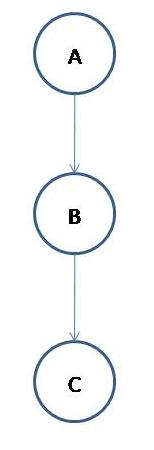
\includegraphics[height=100mm]{figs/verif_case_1.jpg}
\caption{Reference Frame A is a parent to Reference Frame B, who is a parent to
Reference Frame C}
\label{fig:verif_config_1}
\end{center}
\end{figure}

The first is shown above in Figure \ref{fig:verif_config_1}. As shown, this
configuration contains three reference frames: frame A, which is a parent to
frame B, which is a parent to frame C.

\begin{figure}[H]
\begin{center}
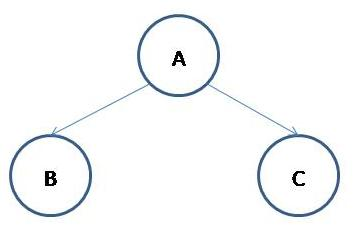
\includegraphics[height=50mm]{figs/verif_case_2.jpg}
\caption{Reference Frame A is a parent to both Reference Frame B and
Reference Frame C}
\label{fig:verif_config_2}
\end{center}
\end{figure}

The second configuration is shown above in Figure \ref{fig:verif_config_2}.
As shown, this configuration contains three reference frames: Frame A, which
is a parent to both Frame B and Frame C. Frame B and C are, thus, siblings
of one another.

The six tests that follow will use these two configurations of reference
frame trees. Three tests will involve the first configuration. A random relative
state of Frame B with respect to A will be specified, and a random relative state
of Frame C with respect to B will be specified. The reference frame model will
then calculate the relative states of Frame A with respect to C, and of Frame
C with respect to Frame A. This will be done both for the complete state, as well
as the position specific version of the algorithm. These results will then
be compared against an independently programmed Matlab solution.

Similarly, three tests will involve the second configuration. A random relative
state of Frame B with respect to A will be specified, and a random relative state
of Frame C with respect to A will be specified. The reference frame model
will then calculate the relative state of Frame B with respect to C, and
of Frame C with respect to Frame A. This will be done both for the complete state,
as well as the position specific version of the algorithm. These results
will then be compared against an independently programmed Matlab solution.

Note that all random relative states were created in Matlab, and the states
themselves will be presented with each test.

\test{Relative State Test 1, Configuration 1}\label{test:refframe_test_1}
\begin{description}
\item[Purpose:] \ \newline

SIM directory: SIM\_REF\_FRAMES
RUN directory: SET\_test\_val/RUN1\_ref\_frame\_ver

The purpose of this test is to demonstrate the relative state and
position calculations associated with \refframesDesc.

\item[Requirements:] \ \newline

By passing this test, the \refframesDesc\ partially satisfies
the Requirement \ref{reqt:refframe_rel_state}

\item[Procedure:] \ \newline

The following relative states were inputted for reference Frames B and
C, configured as shown in \ref{fig:verif_config_1}. \\

\Large{\textbf{$S_{A:B}$:}} \normalsize \\

$x_{A:B}$:  $\left( \begin{array} {ccc} 1848.16 \\ 9048.81 \\ 9797.48;
\end{array} \right) \\ \\$

$v_{A:B}$:   $\left( \begin{array} {ccc}  -408.72 \\ -594.896 \\ 262.212;
\end{array} \right) \\ \\$

$T_{A:B}$:   $\left( \begin{array} {ccc}
 0.02165177281818631 & -0.9708670732541415 & 0.2386384855901647 \\
  -0.1303430129048092 & 0.2339159463811323 & 0.9634801653461872 \\
   -0.9912325154678525 & -0.05196591286176722 & -0.1214810445284236
\end{array} \right) \\ \\$

$w_{A:B}$:   $\left( \begin{array} {ccc}
 11.7418 \\ -29.6676 \\ 31.8778
\end{array} \right)\\ \\$

\Large{\textbf{$S_{B:C}$:}} \normalsize \\

$x_{B:C}$: $\left( \begin{array} {ccc} -2372.84 \\   -4588.49 \\ 9630.89
\end{array} \right)\\ \\$

$v_{B:C}$:  $\left( \begin{array} {ccc}  488.898 \\ 624.06 \\ -679.136
\end{array} \right)\\ \\$

$T_{B:C}$: $\left( \begin{array} {ccc}
 0.7059970877834382 & -0.6729909535450022 & -0.2205703708295675 \\
  0.3550094808358443 & 0.06680598428211491 & 0.9324726424838222 \\
   -0.6128102320930751 & -0.73662754286728 & 0.2860829993749103
\end{array} \right)\\ \\$

$w_{B:C}$:  $\left( \begin{array} {ccc}  -3.77389 \\  88.5168 \\  91.3287
\end{array} \right)\\ \\$


The following relative states will then be calculated:

$S_{A:C}$
$S_{C:A}$

Additionally, the relative positions:

$x_{A:C}$
$x_{C:A}$

will be calculated using the separate, position specific algorithm.

These relative states and positions will then be compared to an
independently programmed Matlab relative state and position calculation.


\item[Results:] \ \newline

The following are the results from the independently programmed Matlab relative state
solution:

$x_{A:C}$: $\left( \begin{array} {ccc}  -7151.589902224503 \\     9778.723254768729 \\     3640.339375024558
\end{array} \right)\\ \\$

$v_{A:C}$:  $\left( \begin{array} {ccc}  144957.2752796087 \\     96815.65534740115 \\    -198952.3536598123
\end{array} \right)\\ \\$

$T_{A:C}$: $\left( \begin{array} {ccc}
 0.3216422806127932 &   -0.8313905014762567 &   -0.4531402402979231 \\
  -0.9253183116582367 &   -0.3774968226845905 &   0.03580741505594964 \\
   -0.2008289457029322 &    0.4077817834554374 &   -0.8907197941270596 \\
\end{array} \right)\\ \\$

$w_{A:C}$:  $\left( \begin{array} {ccc}  17.45051485149649 \\      120.428453505361 \\     115.1068727450524
\end{array} \right)\\ \\$

$x_{C:A}$: $\left( \begin{array} {ccc} 12079.77557590324 \\    -3056.411278357381 \\     -2181.30913023573
\end{array} \right)\\ \\$

$v_{C:A}$:  $\left( \begin{array} {ccc}  -145408.3486105788 \\    -1250726.964369239 \\     1320505.798372557
\end{array} \right)\\ \\$

$T_{C:A}$: $\left( \begin{array} {ccc}
0.3216422806127932 &   -0.9253183116582367 &   -0.2008289457029322 \\
 -0.8313905014762567 &   -0.3774968226845905 &    0.4077817834554374 \\
  -0.4531402402979231 &   0.03580741505594964 &   -0.8907197941270596 \\
\end{array} \right)\\ \\$

$w_{C:A}$:  $\left( \begin{array} {ccc}
 128.9386217750408 \\     13.03106499654173 \\     106.1232688679998
\end{array} \right)\\ \\$

The following are the results from the \refframesDesc\ full relative state calculation:

$x_{A:C}$: $\left( \begin{array} {ccc}  -7151.589902224503 \\     9778.723254768729 \\     3640.339375024558
\end{array} \right)\\ \\$

$v_{A:C}$:  $\left( \begin{array} {ccc}  144957.2752796087 \\     96815.65534740115 \\    -198952.3536598123
\end{array} \right)\\ \\$

$T_{A:C}$: $\left( \begin{array} {ccc}
 0.3216422806127932 &   -0.8313905014762567 &   -0.4531402402979231 \\
  -0.9253183116582367 &   -0.3774968226845905 &   0.03580741505594964 \\
   -0.2008289457029322 &    0.4077817834554374 &   -0.8907197941270596 \\
\end{array} \right)\\ \\$

$w_{A:C}$:  $\left( \begin{array} {ccc}  17.45051485149649 \\      120.428453505361 \\     115.1068727450524
\end{array} \right)\\ \\$

$x_{C:A}$: $\left( \begin{array} {ccc} 12079.77557590324 \\    -3056.411278357381 \\     -2181.30913023573
\end{array} \right)\\ \\$

$v_{C:A}$:  $\left( \begin{array} {ccc}  -145408.3486105788 \\    -1250726.964369239 \\     1320505.798372557
\end{array} \right)\\ \\$

$T_{C:A}$: $\left( \begin{array} {ccc}
0.3216422806127932 &   -0.9253183116582367 &   -0.2008289457029322 \\
 -0.8313905014762567 &   -0.3774968226845905 &    0.4077817834554374 \\
  -0.4531402402979231 &   0.03580741505594964 &   -0.8907197941270596 \\
\end{array} \right)\\ \\$

$w_{C:A}$:  $\left( \begin{array} {ccc}
 128.9386217750408 \\     13.03106499654173 \\     106.1232688679998
\end{array} \right)\\ \\$


The following are the results from the \refframesDesc\ position specific calculation:

$x_{A:C}$: $\left( \begin{array} {ccc}  -7151.589902224503 \\     9778.723254768729 \\     3640.339375024558
\end{array} \right)\\ \\$

$x_{C:A}$: $\left( \begin{array} {ccc} 12079.77557590324 \\    -3056.411278357381 \\     -2181.30913023573
\end{array} \right)\\ \\$

All \refframesDesc\ produced states are a numerical match to the independently programmed Matlab solution.

\end{description}

\test{Relative State Test 2, Configuration 1}\label{test:refframe_test_2}
\begin{description}
\item[Purpose:] \ \newline

SIM directory: SIM\_REF\_FRAMES
RUN directory: SET\_test\_val/RUN2\_ref\_frame\_ver

The purpose of this test is to demonstrate the relative state and
position calculations associated with \refframesDesc.

\item[Requirements:] \ \newline

By passing this test, the \refframesDesc\ partially satisfies
the Requirement \ref{reqt:refframe_rel_state}

\item[Procedure:] \ \newline
$x_{A:B}$:  $\left( \begin{array} {ccc} -8033.64 \\    604.712 \\   -3992.58
\end{array} \right)\\ \\$

$v_{A:B}$:   $\left( \begin{array} {ccc}  627.973 \\   -291.984 \\    431.651
\end{array} \right)\\ \\$

$T_{A:B}$:   $\left( \begin{array} {ccc}\
0.4272687159464157 & -0.3061054736119365 & -0.8507296182679391 \\
0.1149180951186981 & 0.9516978685416249 & -0.2847191571138446 \\
0.8967916568455525 & 0.02388736147296944 & 0.4418077841936113
\end{array} \right)\\ \\$

$w_{A:B}$:   $\left( \begin{array} {ccc}
10.6216 \\     37.241 \\   -19.8118
\end{array} \right)\\ \\$

\Large{\textbf{$S_{B:C}$:}} \normalsize \\

$x_{B:C}$: $\left( \begin{array} {ccc}  -4177.44 \\   -9830.52 \\   -3014.55
\end{array} \right)\\ \\$

$v_{B:C}$:  $\left( \begin{array} {ccc} 698.106 \\   -666.528 \\    178.132
\end{array} \right)\\ \\$

$T_{B:C}$: $\left( \begin{array} {ccc}
 0.6361951982813826 & 0.3331380394803984 & 0.695898495712463 \\
  0.564199301993485 & 0.414337780792221 & -0.7141451890464865 \\
  -0.5262459665534518 & 0.8469611856864128 & 0.07564345726425621

\end{array} \right)\\ \\$
$w_{B:C}$:  $\left( \begin{array} {ccc} -3.26008 \\      56.12 \\    88.1867
\end{array} \right)\\ \\$

The following relative states will then be calculated:

$S_{A:C}$
$S_{C:A}$

Additionally, the relative positions:

$x_{A:C}$
$x_{C:A}$

will be calculated using the separate, position specific algorithm.

These relative states and positions will then be compared to an
independently programmed Matlab relative state and position calculation.

\item[Results:] \ \newline

The following are the results from the independently programmed Matlab relative state
solution:


$x_{A:C}$: $\left( \begin{array} {ccc} -13651.65734631322 \\    -7544.245326498707 \\      1028.37764908716
\end{array} \right)\\ \\$

$v_{A:C}$:  $\left( \begin{array} {ccc}  -71105.87066818211 \\     203306.0472083863 \\     251222.1995609853
\end{array} \right)\\ \\$

$T_{A:C}$: $\left( \begin{array} {ccc}
0.9341858593359342 &    0.1389271085396476 &   -0.3286275075668436 \\
 -0.3517598275083078 &    0.2045608440130484 &   -0.9134658640846932 \\
 -0.05968085093317921 &    0.9689448485901985 &     0.239966823586948 \\
\end{array} \right)\\ \\$

$w_{A:C}$:  $\left( \begin{array} {ccc}
2.116722828998875 \\     91.69155425688828 \\     112.6401743111756
\end{array} \right)\\ \\$

$x_{C:A}$: $\left( \begin{array} {ccc}  14139.23862240651 \\    -2319.459564082803 \\     6248.438600636182
\end{array} \right)\\ \\$

$v_{C:A}$:  $\left( \begin{array} {ccc}  -713453.4736831919 \\     -1416537.83223535 \\     1039837.419066911
\end{array} \right)\\ \\$

$T_{C:A}$: $\left( \begin{array} {ccc}
 0.9341858593359342 &   -0.3517598275083078 &  -0.05968085093317921 \\
  0.1389271085396476 &    0.2045608440130484 &    0.9689448485901985 \\
  -0.3286275075668436 &   -0.9134658640846932 &     0.239966823586948 \\
\end{array} \right)\\ \\$

$w_{C:A}$:  $\left( \begin{array} {ccc} 36.99845422653996 \\    -128.1926885529855 \\     57.42281334830777
\end{array} \right)\\ \\$

The following are the results from the \refframesDesc\ full relative state calculation:

$x_{A:C}$: $\left( \begin{array} {ccc} -13651.65734631322 \\    -7544.245326498707 \\      1028.37764908716
\end{array} \right)\\ \\$

$v_{A:C}$:  $\left( \begin{array} {ccc}  -71105.87066818211 \\     203306.0472083863 \\     251222.1995609853
\end{array} \right)\\ \\$

$T_{A:C}$: $\left( \begin{array} {ccc}
0.9341858593359342 &    0.1389271085396476 &   -0.3286275075668436 \\
 -0.3517598275083078 &    0.2045608440130484 &   -0.9134658640846932 \\
 -0.05968085093317921 &    0.9689448485901985 &     0.239966823586948 \\
\end{array} \right)\\ \\$

$w_{A:C}$:  $\left( \begin{array} {ccc}
2.116722828998875 \\     91.69155425688828 \\     112.6401743111756
\end{array} \right)\\ \\$

$x_{C:A}$: $\left( \begin{array} {ccc}  14139.23862240651 \\    -2319.459564082803 \\     6248.438600636182
\end{array} \right)\\ \\$

$v_{C:A}$:  $\left( \begin{array} {ccc}  -713453.4736831919 \\     -1416537.83223535 \\     1039837.419066911
\end{array} \right)\\ \\$

$T_{C:A}$: $\left( \begin{array} {ccc}
 0.9341858593359342 &   -0.3517598275083078 &  -0.05968085093317921 \\
  0.1389271085396476 &    0.2045608440130484 &    0.9689448485901985 \\
  -0.3286275075668436 &   -0.9134658640846932 &     0.239966823586948 \\
\end{array} \right)\\ \\$

$w_{C:A}$:  $\left( \begin{array} {ccc} 36.99845422653996 \\    -128.1926885529855 \\     57.42281334830777
\end{array} \right)\\ \\$

The following are the results from the \refframesDesc\ position specific calculation:

$x_{A:C}$: $\left( \begin{array} {ccc} -13651.65734631322 \\    -7544.245326498707 \\      1028.37764908716
\end{array} \right)\\ \\$

$x_{C:A}$: $\left( \begin{array} {ccc}  14139.23862240651 \\    -2319.459564082803 \\     6248.438600636182
\end{array} \right)\\ \\$

All \refframesDesc\ produced states are a numerical match to the independently programmed Matlab solution.
\end{description}

\test{Relative State Test 3, Configuration 1}\label{test:refframe_test_3}
\begin{description}
\item[Purpose:] \ \newline

SIM directory: SIM\_REF\_FRAMES
RUN directory: SET\_test\_val/RUN3\_ref\_frame\_ver

The purpose of this test is to demonstrate the relative state and
position calculations associated with \refframesDesc.

\item[Requirements:] \ \newline

By passing this test, the \refframesDesc\ partially satisfies
the Requirement \ref{reqt:refframe_rel_state}

\item[Procedure:] \ \newline
$x_{A:B}$:  $\left( \begin{array} {ccc} 2664.71 \\   -1536.57 \\    2810.05
\end{array} \right)\\ \\$

$v_{A:B}$:   $\left( \begin{array} {ccc}  -875.372 \\   -518.052 \\    943.623
\end{array} \right)\\ \\$

$T_{A:B}$:   $\left( \begin{array} {ccc}
0.8532057436490301 & 0.2501060894816011 & -0.4576973923986534 \\
-0.3517114947196397 & 0.9238850041384419 & -0.1507830348885044 \\
 0.3851480020542523 & 0.2896263854215159 & 0.8762291785721845
\end{array} \right)\\ \\$

$w_{A:B}$:   $\left( \begin{array} {ccc}  -67.6122 \\    28.9065 \\    67.1808
\end{array} \right)\\ \\$

\Large{\textbf{$S_{B:C}$:}} \normalsize \\

$x_{B:C}$: $\left( \begin{array} {ccc}  6021.7 \\    3867.71 \\    9159.91
\end{array} \right)\\ \\$

$v_{B:C}$:  $\left( \begin{array} {ccc}  -460.916 \\     770.16 \\    322.472
\end{array} \right)\\ \\$

$T_{B:C}$: $\left( \begin{array} {ccc}
 -0.9655570135702486 & -0.1962017385355807 & -0.1708933332254907 \\
  0.1197804372000868 & 0.2478810463059914 & -0.9613571832292113 \\
   0.2309811689498931 & -0.9487148489814329 & -0.2158421527706723
\end{array} \right)\\ \\$

$w_{B:C}$:  $\left( \begin{array} {ccc}  17.5874 \\    72.1758 \\   -47.3486
\end{array} \right)\\ \\$

The following relative states will then be calculated:

$S_{A:C}$
$S_{C:A}$

Additionally, the relative positions:

$x_{A:C}$
$x_{C:A}$

will be calculated using the separate, position specific algorithm.

These relative states and positions will then be compared to an
independently programmed Matlab relative state and position calculation.

\item[Results:] \ \newline

The following are the results from the independently programmed Matlab relative state
solution:

$x_{A:C}$: $\left( \begin{array} {ccc} 9970.061996786033 \\     6195.764732474048 \\      7496.92897541955
\end{array} \right)\\ \\$

$v_{A:C}$:  $\left( \begin{array} {ccc}  -525060.1334150368 \\     821188.5121990081 \\    -536983.4183932868
\end{array} \right)\\ \\$

$T_{A:C}$: $\left( \begin{array} {ccc}
 -0.8206316089279889 &    -0.472254751249236 &    0.3217750959144952 \\
  -0.3552500546942768 &  -0.01946300784092403 &   -0.9345686651956066 \\
  0.4476172037220795 &   -0.8812472077960342 &   -0.1517965667718475 \\
\end{array} \right)\\ \\$

$w_{A:C}$:  $\left( \begin{array} {ccc}  65.71857751718055 \\     6.657809933899429 \\    -104.8902192702117
\end{array} \right)\\ \\$

$x_{C:A}$: $\left( \begin{array} {ccc} 8695.402309937857 \\     10668.84819285635 \\     2135.237178517832
\end{array} \right)\\ \\$

$v_{C:A}$:  $\left( \begin{array} {ccc} -1003556.704160732 \\     379994.6857444195 \\     233934.6017263197
\end{array} \right)\\ \\$

$T_{C:A}$: $\left( \begin{array} {ccc}
 -0.8206316089279889 &   -0.3552500546942768 &    0.4476172037220795 \\
  -0.472254751249236 &  -0.01946300784092403 &   -0.8812472077960342 \\
  0.3217750959144952 &   -0.9345686651956066 &   -0.1517965667718475 \\
\end{array} \right)\\ \\$

$w_{C:A}$:  $\left( \begin{array} {ccc} 103.2465959950725 \\    -61.26872137221126 \\    -30.84639621406894
\end{array} \right)\\ \\$

The following are the results from the \refframesDesc\ full relative state calculation:

$x_{A:C}$: $\left( \begin{array} {ccc} 9970.061996786033 \\     6195.764732474048 \\      7496.92897541955
\end{array} \right)\\ \\$

$v_{A:C}$:  $\left( \begin{array} {ccc}  -525060.1334150368 \\     821188.5121990081 \\    -536983.4183932868
\end{array} \right)\\ \\$

$T_{A:C}$: $\left( \begin{array} {ccc}
 -0.8206316089279889 &    -0.472254751249236 &    0.3217750959144952 \\
  -0.3552500546942768 &  -0.01946300784092403 &   -0.9345686651956066 \\
  0.4476172037220795 &   -0.8812472077960342 &   -0.1517965667718475 \\
\end{array} \right)\\ \\$

$w_{A:C}$:  $\left( \begin{array} {ccc}  65.71857751718055 \\     6.657809933899429 \\    -104.8902192702117
\end{array} \right)\\ \\$

$x_{C:A}$: $\left( \begin{array} {ccc} 8695.402309937857 \\     10668.84819285635 \\     2135.237178517832
\end{array} \right)\\ \\$

$v_{C:A}$:  $\left( \begin{array} {ccc} -1003556.704160732 \\     379994.6857444195 \\     233934.6017263197
\end{array} \right)\\ \\$

$T_{C:A}$: $\left( \begin{array} {ccc}
 -0.8206316089279889 &   -0.3552500546942768 &    0.4476172037220795 \\
  -0.472254751249236 &  -0.01946300784092403 &   -0.8812472077960342 \\
  0.3217750959144952 &   -0.9345686651956066 &   -0.1517965667718475 \\
\end{array} \right)\\ \\$

$w_{C:A}$:  $\left( \begin{array} {ccc} 103.2465959950725 \\    -61.26872137221126 \\    -30.84639621406894
\end{array} \right)\\ \\$


The following are the results from the \refframesDesc\ position specific calculation:

$x_{A:C}$: $\left( \begin{array} {ccc} 9970.061996786033 \\     6195.764732474048 \\      7496.92897541955
\end{array} \right)\\ \\$

$x_{C:A}$: $\left( \begin{array} {ccc} 8695.402309937857 \\     10668.84819285635 \\     2135.237178517832
\end{array} \right)\\ \\$

All \refframesDesc\ produced states are a numerical match to the independently programmed Matlab solution.

\end{description}

\test{Relative State Test 1, Configuration 2}\label{test:refframe_test_4}
\begin{description}
\item[Purpose:] \ \newline

SIM directory: SIM\_REF\_FRAMES
RUN directory: SET\_test\_val/RUN1\_ref\_frame\_ver

The purpose of this test is to demonstrate the relative state and
position calculations associated with \refframesDesc.

\item[Requirements:] \ \newline

By passing this test, the \refframesDesc\ partially satisfies
the Requirement \ref{reqt:refframe_rel_state}

\item[Procedure:] \ \newline
$x_{A:B}$:  $\left( \begin{array} {ccc} -7790.52 \\    7150.37 \\   -9037.21
\end{array} \right)\\ \\$

$v_{A:B}$:   $\left( \begin{array} {ccc}  -197.81 \\    30.5409 \\   -744.074
\end{array} \right)\\ \\$

$T_{A:B}$:   $\left( \begin{array} {ccc}
0.9055697770991294 & 0.4006122484928437 & 0.1394747473994526 \\
 -0.4100036383807383 & 0.9109467042835068 & 0.04553151073239373 \\
  -0.1088135805825256 & -0.09841711392093039 & 0.9891782834091561
\end{array} \right)\\ \\$

$w_{A:B}$:   $\left( \begin{array} {ccc}  -60.9867 \\   -61.7666 \\    85.9442
\end{array} \right)\\ \\$

\Large{\textbf{$S_{A:C}$:}} \normalsize \\

$x_{A:C}$: $\left( \begin{array} {ccc}  -5004.72 \\    4710.88 \\    596.189
\end{array} \right)\\ \\$

$v_{A:C}$:  $\left( \begin{array} {ccc}  -521.65 \\     -96.73 \\    818.149
\end{array} \right)\\ \\$

$T_{A:C}$: $\left( \begin{array} {ccc}
0.09641301427589605 & -0.8301616645135473 & 0.5491230658516651 \\
-0.6488031425776438 & 0.3659638227289848 & 0.6671768600865603 \\
 -0.7548238290221164 & -0.4205973029225039 & -0.5033278215186462
\end{array} \right)\\ \\$

$w_{B:C}$:  $\left( \begin{array} {ccc} -65.9605 \\   -51.8595 \\    97.2975
\end{array} \right)\\ \\$

The following relative states will then be calculated:

$S_{B:C}$
$S_{C:B}$

Additionally, the relative positions:

$x_{A:B}$
$x_{B:A}$

will be calculated using the separate, position specific algorithm.

These relative states and positions will then be compared to an
independently programmed Matlab relative state and position calculation.

\item[Results:] \ \newline

The following are the results from the independently programmed Matlab relative state
solution:

$x_{B:C}$: $\left( \begin{array} {ccc} 2889.062603090087 \\    -2925.810301475702 \\     9466.103778667652
\end{array} \right)\\ \\$

$v_{B:C}$:  $\left( \begin{array} {ccc}  333106.2646036395 \\    -825516.6365463276 \\    -355290.0084029901
\end{array} \right)\\ \\$

$T_{B:C}$: $\left( \begin{array} {ccc}
 -0.168675418285182 &   -0.7707603161852675 &    0.6143916814706279 \\
 -0.3478726032834237 &    0.6297627576170896 &    0.6945383509953449 \\
 -0.9222435985959093 &  -0.09657848679962694 &   -0.3743518942604159 \\
\end{array} \right)\\ \\$

$w_{B:C}$:  $\left( \begin{array} {ccc}  -176.6581028286698 \\    -93.86834069564757 \\     67.26095563344904
\end{array} \right)\\ \\$

$x_{C:B}$: $\left( \begin{array} {ccc}  -7583.680047586309 \\    -3726.980016279078 \\     5925.503040873298
\end{array} \right)\\ \\$

$v_{C:B}$:  $\left( \begin{array} {ccc}  -56264.49890069378 \\     345818.1552020046 \\     147940.7284172714
\end{array} \right)\\ \\$

$T_{C:B}$: $\left( \begin{array} {ccc}
-0.168675418285182 &   -0.3478726032834237 &   -0.9222435985959093 \\
-0.7707603161852675 &    0.6297627576170896 &  -0.09657848679962694 \\
0.6143916814706279 &    0.6945383509953449 &   -0.3743518942604159 \\
\end{array} \right)\\ \\$

$w_{C:B}$:  $\left( \begin{array} {ccc} -0.421117663390973 \\    -70.55030878770818 \\     198.9116975508892
\end{array} \right)\\ \\$

The following are the results from the \refframesDesc\ full relative state calculation:

$x_{B:C}$: $\left( \begin{array} {ccc} 2889.062603090087 \\    -2925.810301475702 \\     9466.103778667652
\end{array} \right)\\ \\$

$v_{B:C}$:  $\left( \begin{array} {ccc}  333106.2646036395 \\    -825516.6365463276 \\    -355290.0084029901
\end{array} \right)\\ \\$

$T_{B:C}$: $\left( \begin{array} {ccc}
 -0.168675418285182 &   -0.7707603161852675 &    0.6143916814706279 \\
 -0.3478726032834237 &    0.6297627576170896 &    0.6945383509953449 \\
 -0.9222435985959093 &  -0.09657848679962694 &   -0.3743518942604159 \\
\end{array} \right)\\ \\$

$w_{B:C}$:  $\left( \begin{array} {ccc}  -176.6581028286698 \\    -93.86834069564757 \\     67.26095563344904
\end{array} \right)\\ \\$

$x_{C:B}$: $\left( \begin{array} {ccc}  -7583.680047586309 \\    -3726.980016279078 \\     5925.503040873298
\end{array} \right)\\ \\$

$v_{C:B}$:  $\left( \begin{array} {ccc}  -56264.49890069378 \\     345818.1552020046 \\     147940.7284172714
\end{array} \right)\\ \\$

$T_{C:B}$: $\left( \begin{array} {ccc}
-0.168675418285182 &   -0.3478726032834237 &   -0.9222435985959093 \\
-0.7707603161852675 &    0.6297627576170896 &  -0.09657848679962694 \\
0.6143916814706279 &    0.6945383509953449 &   -0.3743518942604159 \\
\end{array} \right)\\ \\$

$w_{C:B}$:  $\left( \begin{array} {ccc} -0.421117663390973 \\    -70.55030878770818 \\     198.9116975508892
\end{array} \right)\\ \\$


The following are the results from the \refframesDesc\ position specific calculation:

$x_{B:C}$: $\left( \begin{array} {ccc} 2889.062603090087 \\    -2925.810301475702 \\     9466.103778667652
\end{array} \right)\\ \\$

$x_{C:B}$: $\left( \begin{array} {ccc}  -7583.680047586309 \\    -3726.980016279078 \\     5925.503040873298
\end{array} \right)\\ \\$

All \refframesDesc\ produced states are a numerical match to the independently programmed Matlab solution.

\end{description}

\test{Relative State Test 2, Configuration 2}\label{test:refframe_test_5}
\begin{description}
\item[Purpose:] \ \newline

SIM directory: SIM\_REF\_FRAMES
RUN directory: SET\_test\_val/RUN2\_ref\_frame\_ver

The purpose of this test is to demonstrate the relative state and
position calculations associated with \refframesDesc.

\item[Requirements:] \ \newline

By passing this test, the \refframesDesc\ partially satisfies
the Requirement \ref{reqt:refframe_rel_state}

\item[Procedure:] \ \newline
$x_{A:B}$:  $\left( \begin{array} {ccc}  -4282.53 \\    4820.22 \\    1206.12
\end{array} \right)\\ \\$

$v_{A:B}$:   $\left( \begin{array} {ccc}  -582.986 \\    251.806 \\   -290.441
\end{array} \right)\\ \\$

$T_{A:B}$:   $\left( \begin{array} {ccc}
0.9945282144718409 & -0.1036578778650371 & -0.01298749305944376 \\
0.09724675025241425 & 0.9640168959942612 & -0.2474156296658203 \\
0.03816674186771286 & 0.2447988329100178 & 0.9688223940542955
\end{array} \right)\\ \\$

$w_{A:B}$:   $\left( \begin{array} {ccc}  -98.2663 \\    73.0249 \\   -34.3877
\end{array} \right)\\ \\$

\Large{\textbf{$S_{B:C}$:}} \normalsize \\

$x_{A:C}$: $\left( \begin{array} {ccc} 1614.85 \\   -1787.66 \\    4228.86
\end{array} \right)\\ \\$

$v_{A:C}$:  $\left( \begin{array} {ccc} 695.949 \\    699.888 \\    638.531
\end{array} \right)\\ \\$

$T_{A:C}$: $\left( \begin{array} {ccc}
 0.5617023094980858 & -0.1323969387778994 & 0.8166771492497862 \\
  0.7140778066635471 & 0.5761043624264366 & -0.3977394242765062 \\
   -0.4178317861712943 & 0.8065821806830784 & 0.4181408665383421
\end{array} \right)\\ \\$

$w_{A:C}$:  $\left( \begin{array} {ccc}  -53.0864 \\   -65.4446 \\   -40.7619
\end{array} \right)\\ \\$

The following relative states will then be calculated:

$S_{B:C}$
$S_{C:B}$

Additionally, the relative positions:

$x_{B:C}$
$x_{C:B}$

will be calculated using the separate, position specific algorithm.

These relative states and positions will then be compared to an
independently programmed Matlab relative state and position calculation.

\item[Results:] \ \newline

The following are the results from the independently programmed Matlab relative state
solution:

$x_{B:C}$: $\left( \begin{array} {ccc} 6510.811804678263 \\    -6544.480047115037 \\     1535.980671550045
\end{array} \right)\\ \\$

$v_{B:C}$:  $\left( \begin{array} {ccc} 114098.2062696465 \\     73283.19432999958 \\    -166591.9470886627
\end{array} \right)\\ \\$

$T_{B:C}$: $\left( \begin{array} {ccc}
0.5617461918316968 &   -0.2750678528671711 &    0.7802428418650378 \\
0.6556184084294097 &    0.7232230354607804 &   -0.2170551623605903 \\
-0.5045846990259157 &     0.633471481045468 &    0.5866073339219234 \\
\end{array} \right)\\ \\$

$w_{B:C}$:  $\left( \begin{array} {ccc} 49.03187903243332 \\    -61.29672244068031 \\    -116.4326859493806
\end{array} \right)\\ \\$

$x_{C:B}$: $\left( \begin{array} {ccc}  -6656.037735922825 \\     797.9031862664995 \\     6529.979956302859
\end{array} \right)\\ \\$

$v_{C:B}$:  $\left( \begin{array} {ccc}  393410.1500972123 \\    -618767.7848463297 \\      477744.058501485
\end{array} \right)\\ \\$

$T_{C:B}$: $\left( \begin{array} {ccc}
 0.5617461918316968 &    0.6556184084294097 &   -0.5045846990259157 \\
  -0.2750678528671711 &    0.7232230354607804 &     0.633471481045468 \\
  0.7802428418650378 &   -0.2170551623605903 &    0.5866073339219234 \\
\end{array} \right)\\ \\$

$w_{C:B}$:  $\left( \begin{array} {ccc} -46.10636351287094 \\     131.5750813652961 \\      16.7387248063523
\end{array} \right)\\ \\$

The following are the results from the \refframesDesc\ full relative state calculation:

$x_{B:C}$: $\left( \begin{array} {ccc} 6510.811804678263 \\    -6544.480047115037 \\     1535.980671550045
\end{array} \right)\\ \\$

$v_{B:C}$:  $\left( \begin{array} {ccc} 114098.2062696465 \\     73283.19432999958 \\    -166591.9470886627
\end{array} \right)\\ \\$

$T_{B:C}$: $\left( \begin{array} {ccc}
0.5617461918316968 &   -0.2750678528671711 &    0.7802428418650378 \\
0.6556184084294097 &    0.7232230354607804 &   -0.2170551623605903 \\
-0.5045846990259157 &     0.633471481045468 &    0.5866073339219234 \\
\end{array} \right)\\ \\$

$w_{B:C}$:  $\left( \begin{array} {ccc} 49.03187903243332 \\    -61.29672244068031 \\    -116.4326859493806
\end{array} \right)\\ \\$

$x_{C:B}$: $\left( \begin{array} {ccc}  -6656.037735922825 \\     797.9031862664995 \\     6529.979956302859
\end{array} \right)\\ \\$

$v_{C:B}$:  $\left( \begin{array} {ccc}  393410.1500972123 \\    -618767.7848463297 \\      477744.058501485
\end{array} \right)\\ \\$

$T_{C:B}$: $\left( \begin{array} {ccc}
 0.5617461918316968 &    0.6556184084294097 &   -0.5045846990259157 \\
  -0.2750678528671711 &    0.7232230354607804 &     0.633471481045468 \\
  0.7802428418650378 &   -0.2170551623605903 &    0.5866073339219234 \\
\end{array} \right)\\ \\$

$w_{C:B}$:  $\left( \begin{array} {ccc} -46.10636351287094 \\     131.5750813652961 \\      16.7387248063523
\end{array} \right)\\ \\$


The following are the results from the \refframesDesc\ position specific calculation:

$x_{B:C}$: $\left( \begin{array} {ccc} 6510.811804678263 \\    -6544.480047115037 \\     1535.980671550045
\end{array} \right)\\ \\$

$x_{C:B}$: $\left( \begin{array} {ccc}  -6656.037735922825 \\     797.9031862664995 \\     6529.979956302859
\end{array} \right)\\ \\$

All \refframesDesc\ produced states are a numerical match to the independently programmed Matlab solution.

\end{description}

\test{Relative State Test 3, Configuration 2}\label{test:refframe_test_6}
\begin{description}
\item[Purpose:] \ \newline

SIM directory: SIM\_REF\_FRAMES
RUN directory: SET\_test\_val/RUN3\_ref\_frame\_ver

The purpose of this test is to demonstrate the relative state and
position calculations associated with \refframesDesc.

\item[Requirements:] \ \newline

By passing this test, the \refframesDesc\ partially satisfies
the Requirement \ref{reqt:refframe_rel_state}

\item[Procedure:] \ \newline
$x_{A:B}$:  $\left( \begin{array} {ccc}  -2874.98 \\   -911.135 \\    5762.09
\end{array} \right)\\ \\$

$v_{A:B}$:   $\left( \begin{array} {ccc}  -644.443 \\   -647.618 \\    679.017
\end{array} \right)\\ \\$

$T_{A:B}$:   $\left( \begin{array} {ccc}
 -0.1766406884173243 & -0.3584722730823265 & -0.9166764405321235 \\
  -0.07753089247582201 & 0.9334947713181074 & -0.3501092295750815 \\
   0.9812171155801128 & 0.009227207212613942 & -0.1926858342995125
\end{array} \right)\\ \\$

$w_{A:B}$:   $\left( \begin{array} {ccc}  -70.9282 \\    23.6231 \\    11.9396
\end{array} \right)\\ \\$

\Large{\textbf{$S_{B:C}$:}} \normalsize \\

$x_{A:C}$: $\left( \begin{array} {ccc}  -2564.41 \\   -6134.61 \\    5822.49
\end{array} \right)\\ \\$

$v_{A:C}$:  $\left( \begin{array} {ccc}  -318.074 \\    119.215 \\   -939.829
\end{array} \right)\\ \\$

$T_{A:C}$: $\left( \begin{array} {ccc}
 -0.9774834677306422 & 0.1620640475981063 & -0.1351344322865095 \\
  0.04508295495462142 & 0.786020216558487 & 0.6165547391220908 \\
   0.2061397523182708 & 0.5965798049192318 & -0.7756280931456088
\end{array} \right)\\ \\$

$w_{A:C}$:  $\left( \begin{array} {ccc} -54.4716 \\   -64.7311 \\   -54.3886
\end{array} \right)\\ \\$

The following relative states will then be calculated:

$S_{B:C}$
$S_{C:B}$

Additionally, the relative positions:

$x_{B:C}$
$x_{C:B}$

will be calculated using the separate, position specific algorithm.

These relative states and positions will then be compared to an
independently programmed Matlab relative state and position calculation.

\item[Results:] \ \newline

The following are the results from the independently programmed Matlab relative state
solution:

$x_{B:C}$: $\left( \begin{array} {ccc}  1762.244401028797 \\    -4921.311967353402 \\     244.9002889991167
\end{array} \right)\\ \\$

$v_{B:C}$:  $\left( \begin{array} {ccc}  -63392.38080684067 \\    -37153.52608672214 \\    -306790.8805049965
\end{array} \right)\\ \\$

$T_{B:C}$: $\left( \begin{array} {ccc}
 0.2384424355108056 &    0.2743829186618951 &   -0.9315896193572873  \\
 -0.8549111415691051 &    0.5143889358696943 &  -0.06731242586516778 \\
 0.4607300130973512 &    0.8124764837220977 &    0.3572251648888851 \\
\end{array} \right)\\ \\$

$w_{B:C}$:  $\left( \begin{array} {ccc}  -32.91827495216602 \\    -136.7161862625254 \\    -45.16818828635127
\end{array} \right)\\ \\$

$x_{C:B}$: $\left( \begin{array} {ccc} 1158.276661310729 \\     4054.515631124612 \\     3099.046810448993
\end{array} \right)\\ \\$

$v_{C:B}$:  $\left( \begin{array} {ccc} -19938.73745623053 \\    -105432.3449651296 \\     144099.0541189501
\end{array} \right)\\ \\$

$T_{C:B}$: $\left( \begin{array} {ccc}
0.2384424355108056 &   -0.8549111415691051 &    0.4607300130973512 \\
 0.2743829186618951 &    0.5143889358696943 &    0.8124764837220977 \\
  -0.9315896193572873 &  -0.06731242586516778 &    0.3572251648888851 \\
\end{array} \right)\\ \\$

$w_{C:B}$:  $\left( \begin{array} {ccc}  -88.2207372355069 \\     116.0555967214257 \\    -23.73380787662757
\end{array} \right)\\ \\$

The following are the results from the \refframesDesc\ full relative state calculation:

$x_{B:C}$: $\left( \begin{array} {ccc}  1762.244401028797 \\    -4921.311967353402 \\     244.9002889991167
\end{array} \right)\\ \\$

$v_{B:C}$:  $\left( \begin{array} {ccc}  -63392.38080684067 \\    -37153.52608672214 \\    -306790.8805049965
\end{array} \right)\\ \\$

$T_{B:C}$: $\left( \begin{array} {ccc}
 0.2384424355108056 &    0.2743829186618951 &   -0.9315896193572873  \\
 -0.8549111415691051 &    0.5143889358696943 &  -0.06731242586516778 \\
 0.4607300130973512 &    0.8124764837220977 &    0.3572251648888851 \\
\end{array} \right)\\ \\$

$w_{B:C}$:  $\left( \begin{array} {ccc}  -32.91827495216602 \\    -136.7161862625254 \\    -45.16818828635127
\end{array} \right)\\ \\$

$x_{C:B}$: $\left( \begin{array} {ccc} 1158.276661310729 \\     4054.515631124612 \\     3099.046810448993
\end{array} \right)\\ \\$

$v_{C:B}$:  $\left( \begin{array} {ccc} -19938.73745623053 \\    -105432.3449651296 \\     144099.0541189501
\end{array} \right)\\ \\$

$T_{C:B}$: $\left( \begin{array} {ccc}
0.2384424355108056 &   -0.8549111415691051 &    0.4607300130973512 \\
 0.2743829186618951 &    0.5143889358696943 &    0.8124764837220977 \\
  -0.9315896193572873 &  -0.06731242586516778 &    0.3572251648888851 \\
\end{array} \right)\\ \\$

$w_{C:B}$:  $\left( \begin{array} {ccc}  -88.2207372355069 \\     116.0555967214257 \\    -23.73380787662757
\end{array} \right)\\ \\$


The following are the results from the \refframesDesc\ position specific calculation:

$x_{B:C}$: $\left( \begin{array} {ccc}  1762.244401028797 \\    -4921.311967353402 \\     244.9002889991167
\end{array} \right)\\ \\$

$x_{C:B}$: $\left( \begin{array} {ccc} 1158.276661310729 \\     4054.515631124612 \\     3099.046810448993
\end{array} \right)\\ \\$

All \refframesDesc\ produced states are a numerical match to the independently programmed Matlab solution.

\end{description}

\section{Metrics}
\subsection{Code Metrics}

Table~\ref{tab:coarse_metrics} presents coarse metrics on the
source files that comprise the model.

\input{coarse_metrics}

Table~\ref{tab:metrix_metrics} presents the extended cyclomatic
complexity
(ECC) of the methods defined in the model.
\input{metrix_metrics}


\section{Requirements Traceability}\label{sec:traceability}

\begin{longtable}[c]{||p{3in}|p{3in}|}
\caption{Requirements Traceability} \\[6pt]
\hline
{\bf Requirement} & {\bf Inspection and Testing} \\
\hline \hline
\endfirsthead
\hline
\endfoot
\caption[]{Requirements Traceability (continued)} \\[6pt]
\hline
{\bf Requirement} & {\bf Inspection and Testing} \\
\hline \hline
\endhead

\ref{reqt:toplevel} - Top-level Requirements &
  Inspection~\ref{inspect:TLI} \\
  \hline

\ref{reqt:refframe_rep} - Reference Frame Representation Requirement &
   Inspection~\ref{inspect:refframe_representation} \\
\hline

\ref{reqt:refframe_state} - Reference Frame State Requirement &
   Inspection~\ref{inspect:refframe_state} \\
\hline

\ref{reqt:refframe_tree_struct} - Reference Frame Tree Structure &
   Inspection~\ref{inspect:refframe_struct} \\
\hline

\ref{reqt:refframe_manager} - Reference Frame Manager Utility &
   Inspection~\ref{inspect:refframe_manager} \\
\hline
\ref{reqt:refframe_search_registry} - Searchable Registry &
   Inspection~\ref{inspect:refframe_manager} \\
\hline
\ref{reqt:refframe_tree_build} - Tree Building Functionality &
   Inspection~\ref{inspect:refframe_manager} \\
\hline
\ref{reqt:refframe_subscription_mechanism} - Subscription Mechanism Access &
   Inspection~\ref{inspect:refframe_manager} \\
\hline

\ref{reqt:refframe_rel_state} - Reference Frame Relative State Calculation &

   Test~\ref{test:refframe_test_1} \\
   &Test~\ref{test:refframe_test_2} \\
   &Test~\ref{test:refframe_test_3} \\
   &Test~\ref{test:refframe_test_4} \\
   &Test~\ref{test:refframe_test_5} \\
   &Test~\ref{test:refframe_test_6} \\
\hline

\ref{reqt:refframe_active_inactive} - Reference Frame Active/Inactive Functionality &

   Inspection~\ref{inspect:refframe_active_inactive} \\
\hline

\ref{reqt:refframe_subscription} - Reference Frame Subscription Functionality &

   Inspection~\ref{inspect:refframe_subscribe} \\
\hline

\end{longtable}


%%% or for a document with multiple parts make as many copies of Chapters.tex
%%% as you have parts and use this format
%\hyperdef{part}{part1}{\part{Part 1 Title}}\label{pt1:title}
%\include{ref_framesChapters1}
%\hyperdef{part}{part2}{\part{Part 2 Title}}\label{pt2:title}
%\include{ref_framesChapters2}
%%% etc.

%%%%%%%%%%%%%%%%%%%%%%%%%%%%%%%%%%%%%%%%%%%%%%%%%%%%%%%%%%%%%%%%%%%%%%%%%
% Bibliography
%%%%%%%%%%%%%%%%%%%%%%%%%%%%%%%%%%%%%%%%%%%%%%%%%%%%%%%%%%%%%%%%%%%%%%%%%
\newpage
\pdfbookmark{Bibliography}{bibliography}
\bibliography{dynenv,ref_frames}
\bibliographystyle{plain}

%\pagebreak
%\appendix

\end{document}
